%%%%%%%%%%%%%%%%%%%%%%%%%%%%%%%%%%%%%%%%%
% Masters/Doctoral Thesis 
% LaTeX Template
% Version 2.5 (27/8/17)
%
% This template was downloaded from:
% http://www.LaTeXTemplates.com
%
% Version 2.x major modifications by:
% Vel (vel@latextemplates.com)
%
% This template is based on a template by:
% Steve Gunn (http://users.ecs.soton.ac.uk/srg/softwaretools/document/templates/)
% Sunil Patel (http://www.sunilpatel.co.uk/thesis-template/)
%
% Template license:
% CC BY-NC-SA 3.0 (http://creativecommons.org/licenses/by-nc-sa/3.0/)
%
%%%%%%%%%%%%%%%%%%%%%%%%%%%%%%%%%%%%%%%%%

%----------------------------------------------------------------------------------------
%	PACKAGES AND OTHER DOCUMENT CONFIGURATIONS
%----------------------------------------------------------------------------------------
\documentclass[
11pt, % The default document font size, options: 10pt, 11pt, 12pt
%oneside, % Two side (alternating margins) for binding by default, uncomment to switch to one side
ngerman, % ngerman for German
singlespacing, % Single line spacing, alternatives: onehalfspacing or doublespacing
%draft, % Uncomment to enable draft mode (no pictures, no links, overfull hboxes indicated)
%nolistspacing, % If the document is onehalfspacing or doublespacing, uncomment this to set spacing in lists to single
%liststotoc, % Uncomment to add the list of figures/tables/etc to the table of contents
%toctotoc, % Uncomment to add the main table of contents to the table of contents
%parskip, % Uncomment to add space between paragraphs
%nohyperref, % Uncomment to not load the hyperref package
headsepline, % Uncomment to get a line under the header
%chapterinoneline, % Uncomment to place the chapter title next to the number on one line
%consistentlayout, % Uncomment to change the layout of the declaration, abstract and acknowledgements pages to match the default layout
]{MastersDoctoralThesis} % The class file specifying the document structure
\usepackage{float}
\usepackage{caption}
\usepackage{fancyvrb}
\usepackage{enumitem}
\usepackage{capt-of}

\usepackage{pgfplots}
\pgfplotsset{width=7cm,compat=1.8}
\usepackage[utf8]{inputenc} % Required for inputting international characters
\usepackage[T1]{fontenc} % Output font encoding for international characters
\usepackage[colorlinks]{hyperref}
\usepackage{mathpazo} % Use the Palatino font by default
\usepackage{graphicx}
\usepackage{placeins}
\usepackage[backend=bibtex,style=authoryear,natbib=true]{biblatex} % Use the bibtex backend with the authoryear citation style (which resembles APA)

\addbibresource{example.bib} % The filename of the bibliography

\usepackage[autostyle=true]{csquotes} % Required to generate language-dependent quotes in the bibliography

%----------------------------------------------------------------------------------------
%	MARGIN SETTINGS
%----------------------------------------------------------------------------------------

\geometry{
	paper=a4paper, % Change to letterpaper for US letter
	inner=2.5cm, % Inner margin
	outer=3.8cm, % Outer margin
	bindingoffset=.5cm, % Binding offset
	top=1.5cm, % Top margin
	bottom=3cm, % Bottom margin
	%showframe, % Uncomment to show how the type block is set on the page
}

%----------------------------------------------------------------------------------------
%	THESIS INFORMATION
%----------------------------------------------------------------------------------------

\thesistitle{Evaluierung von temporalen Graphdatenbanken am Beispiel von Neo4j} % Your thesis title, this is used in the title and abstract, print it elsewhere with \ttitle
\supervisor{Prof. Dr. Ralf Möller \textsc{Smith}} % Your supervisor's name, this is used in the title page, print it elsewhere with \supname
\examiner{} % Your examiner's name, this is not currently used anywhere in the template, print it elsewhere with \examname
\degree{Bachelor of Science} % Your degree name, this is used in the title page and abstract, print it elsewhere with \degreename
\author{Ove Folger} % Your name, this is used in the title page and abstract, print it elsewhere with \authorname
\addresses{} % Your address, this is not currently used anywhere in the template, print it elsewhere with \addressname

\subject{Graphdatabases} % Your subject area, this is not currently used anywhere in the template, print it elsewhere with \subjectname
\keywords{} % Keywords for your thesis, this is not currently used anywhere in the template, print it elsewhere with \keywordnames
\university{\href{https://www.uni-luebeck.de/universitaet/universitaet.html}{Universität zu Lübeck}} % Your university's name and URL, this is used in the title page and abstract, print it elsewhere with \univname
\department{\href{https://www.ifis.uni-luebeck.de/}{Institut für Informationssysteme}} % Your department's name and URL, this is used in the title page and abstract, print it elsewhere with \deptname
\group{\href{https://www.ifis.uni-luebeck.de/}{Institut für Informationssysteme}} % Your research group's name and URL, this is used in the title page, print it elsewhere with \groupname
\faculty{\href{https://www.uni-luebeck.de/structure/sektionen/informatiktechnik.html}{Sektion Informatik/Technik}} % Your faculty's name and URL, this is used in the title page and abstract, print it elsewhere with \facname

\AtBeginDocument{
\hypersetup{pdftitle=\ttitle} % Set the PDF's title to your title
\hypersetup{pdfauthor=\authorname} % Set the PDF's author to your name
\hypersetup{pdfkeywords=\keywordnames} % Set the PDF's keywords to your keywords
}

\begin{document}
\frontmatter % Use roman page numbering style (i, ii, iii, iv...) for the pre-content pages

\pagestyle{plain} % Default to the plain heading style until the thesis style is called for the body content

%----------------------------------------------------------------------------------------
%	TITLE PAGE
%----------------------------------------------------------------------------------------

\begin{titlepage}

	\Large
	\title{Evaluierung von temporalen Graphdatenbanken am Beispiel von Neo4j }
	\includegraphics[width=8cm]{Figures/ifis_logo.png}
	\vskip 44pt
		 \noindent {\LARGE Evaluierung von temporalen Graphdatenbanken am Beispiel von Neo4j \par}
		\vskip 20pt
	\noindent	\textbf{Bachelorarbeit}
		\vskip 20pt
	 \noindent	im Rahmen des Studiengangs \\
		\textbf{Medieninformatik} \\
		der Universität zu Lübeck
		\vskip 20pt
		\noindent vorgelegt von \\
		\textbf{Ove Folger}
		\vskip 20pt
	\noindent	ausgegeben und betreut von \\
		\textbf{Prof. Dr. Ralf Möller}
		\vfill
		Lübeck, den \today
		\vskip 20pt


\end{titlepage}

%----------------------------------------------------------------------------------------
%	DECLARATION PAGE
%----------------------------------------------------------------------------------------
\begin{declaration}

	\bigskip\noindent Hiermit erkl{\"a}re ich an Eides statt, dass
	ich die vorliegende Arbeit selbst\-st{\"a}n\-dig verfasst und keine
	anderen als die angegebenen Quellen und Hilfsmittel verwendet habe.\par
	\bigskip\noindent Luebeck, \today
	\vskip 10mm
	\hfill\rule{18em}{.3pt}%
\end{declaration}





%----------------------------------------------------------------------------------------
%	ABSTRACT PAGE
%----------------------------------------------------------------------------------------

\begin{abstract}
Durch das steigende Interesse an der Analyse von Netzwerken werden Datenbanken des NoSQL-Ansatzes weiterentwickelt und für diese Analyse genutzt \parencite{angles2018property}. Eine Untergruppe dieses Ansatzes stellen die Graphdatenbanken dar, einer der populärsten Vertreter dieser Gruppe ist Neo4j. In dieser Arbeit wird beschrieben, wie sich verschiedene Arten von Anfragen auf dem System Neo4j verhalten. Zu diesem Zweck wurden mehrere Anfragen mit semantisch gleichen Vergleichsanfragen an das System gestellt und die Differenz in den Bearbeitungszeiten wird betrachtet. Jeder Anfrage wird eine oder mehreren Kategorien zugeordnet, um so eine Korrelation zwischen Kategorie und Bearbeitungszeit einer Anfrage zu erkennen. Nach Ausführen der Anfragen konnte keine Korrelation festgestellt werden. \newline
Für eine Einordnung der Performanz von Neo4j wurden alle aufgestellten Anfragen auf dem Datenbankmanagementsystem OrientDB ausgeführt\footnote{http://orientdb.com/docs/3.0.x/misc/Overview.html (5.09.19)}. Die benötigten Zeiten für das Bearbeiten der Anfragen auf dem System OrientDB wurden mit den Bearbeitungszeiten der Anfragen auf Neo4j verglichen. Die Analyse zeigt, dass Neo4j bei den meisten Anfragen eine signifikant schnellere Bearbeitungszeit aufweist und so das performantere System darstellt. Unter Berücksichtigung der Limitierungen werden die Nutzungsvielfalt und gute Performanz als Stärke und die erforderlichen technischen Kenntnisse und schlechte Speicherverwaltung als Schwäche von Neo4j hervorgehoben. \newline
\begin{center}
\textbf{Evaluation of temporal graph databases using the example of Neo4j}
\end{center}
Due to the increasing interest in the analysis of networks, databases of the NoSQL approach are further developed and used for this analysis  \parencite{han2011survey}. A subset of this approach is represented by the graph databases, one of the most popular members of this group is Neo4j. This work describes how different types of queries behave on the system Neo4j. For this purpose, several queries with semantically equal comparison-queries were made to the system and the difference in the processing times was considered. Each query has been assigned one or more categories to identify a potential relationship between the category and the processing time of a request. After the execution of all queries, no general connection could be established. \newline
To rank the performance of Neo4j, all queries that were made were run on the Database Management System OrientDB \footnotemark[1]. The times needed to process requests on the System OrientDB were compared to the times of requests on Neo4j. The analysis showed that Neo4j has a significantly faster turnaround time for all queries and thus represents the more efficient system. Taking into account these limitations, the versatility and good performance are highlighted as strengths and the required technical knowledge and poor memory management are highlighted as weaknesses of Neo4j.
\end{abstract}




%----------------------------------------------------------------------------------------
%	LIST OF CONTENTS/FIGURES/TABLES PAGES
%----------------------------------------------------------------------------------------

{
	\setcounter{tocdepth}{1}
	\hypersetup{linkcolor=black}
	\tableofcontents
}


\listoffigures % Prints the list of figures


\listoftables % Prints the list of tables
%----------------------------------------------------------------------------------------
%	ABBREVIATIONS
%----------------------------------------------------------------------------------------

\begin{abbreviations}{ll} % Include a list of abbreviations (a table of two columns)
	
	\textbf{SQL} & \textbf{S}tructured \textbf{Q}uery \textbf{L}anguage\\
	\textbf{NoSQL} & \textbf{N}ot \textbf{o}nly \textbf{SQL}\\
	\textbf{GDB} & \textbf{G}raph \textbf{D}ata\textbf{b}ase \\
	\textbf{API} & \textbf{A}pplication \textbf{P}rogramming \textbf{I}nterface \\
	\textbf{DBMS} & \textbf{D}ata\textbf{b}ase\textbf{m}anagement\textbf{s}ystem \\
	\textbf{UDF} & \textbf{U}ser \textbf{D}efined \textbf{F}unctions \\
	\textbf{APOC} & \textbf{A}wesome \textbf{P}rocedures \textbf{o}n \textbf{C}ypher\\
	\textbf{ACID} & \textbf{A}tomicity \textbf{C}onsistency \textbf{I}solation \textbf{D}urability\\
	\textbf{CAP} & \textbf{C}onsistency \textbf{A}vailibility \textbf{P}artition Tolerance  \\
	\textbf{LFU} &\textbf{L}east \textbf{F}requently \textbf{U}sed \\
	\textbf{ASB} & \textbf{A}bstrakter \textbf{S}yntax \textbf{B}aum\\
	
\end{abbreviations}
%----------------------------------------------------------------------------------------
%	DEDICATION
%----------------------------------------------------------------------------------------
\begin{acknowledgements}
An dieser Stelle möchte ich all jenen danken, die durch ihre fachliche und persönliche Unterstützung zum Gelingen dieser Bachelorarbeit beigetragen haben. \newline \newline
Ebenso gilt mein Dank Melf und Lasse für das Korrekturlesen. Zuletzt möchte ich noch all denjenigen danken, die in der Zeit der Erstellung dieser Arbeit für mich da waren, insbesondere meinen Freunden. \newline \newline
Schließlich danke ich meinen Freunden während der Studienzeit für drei sehr schöne Jahre in Lübeck.
\end{acknowledgements}
%----------------------------------------------------------------------------------------
%	THESIS CONTENT - CHAPTERS
%----------------------------------------------------------------------------------------

\mainmatter % Begin numeric (1,2,3...) page numbering

\pagestyle{thesis} % Return the page headers back to the "thesis" style
% Include the chapters of the thesis as separate files from the Chapters folder
% Uncomment the lines as you write the chapters
% Chapter 0

\chapter{Einführungs} % Main chapter title

\label{Kaptiel1} % For referencing the chapter elsewhere, use \ref{Chapter1} 

%----------------------------------------------------------------------------------------

% Define some commands to keep the formatting separated from the content 
\newcommand{\keyword}[1]{\textit{#1}}
\newcommand{\tabhead}[1]{\textbf{#1}}
\newcommand{\code}[1]{\texttt{#1}}
\newcommand{\file}[1]{\texttt{\bfseries#1}}
\newcommand{\option}[1]{\texttt{\itshape#1}}

Um Daten in einer Datenbank abzulegen, ist ein Datenmodell nötig, welches  das allgemeine Verhalten der Datenbank definiert. Dieses ist durch folgende Eigenschaften definiert: ein Liste von Datenstrukturtypen, ein Liste von Operatoren, die auf die Daten angewandt werden können und Regeln zur Vollständigkeit der Datenbank \parencite{codd1981data}. Zwei dieser Datenmodelle sind der Relationale-Ansatz und die NoSQL-Bewegung. Die meisten Datenbanken werden heutzutage nach dem relationalen Datenmodell verwaltet und mittels Structured Query Language (SQL) bearbeitet \parencite{miller2013graph}. Dieser Ansatz wurde über viele Jahre lang optimiert und gilt für viele Daten als performanteste Implementierung \parencite{miller2013graph}. Die Datenstruktur wird eine Tabelle verwendet, eine Reihe bildet ein Objekt und die Spalten bilden die dazugehörigen Attribute \parencite{miller2013graph}. Die Möglichkeiten der Operationen, mit denen die Daten verändert oder angefragt werden, sind durch den SQL-Standard bzw. die Implementierung des  Standards limitiert. Die Regeln zur Vollständigkeit der Datenbank sind ebenfalls im Standard festgehalten. \newline 
Als eine Alternative zu diesem relationalen Datenmodell gibt es die NoSQL-Bewegung, welche erstmals 1998 erwähnt wurde \parencite{strauch2011nosql}. Diese Bewegung versuchte zunächst den Gebrauch von SQL als Anfragesprache zu vermeiden und brachte in den folgenden Jahren weitere Datenmodelle hervor. Eines dieser Modelle ist das Darstellen von Daten in einem Graphen als Datenstruktur \parencite{miller2013graph}. Die sogenannten Graphdatenbanken (GDB) werden besonders zum Darstellen von Netzwerken verwendet \parencite{han2011survey}. Da das relationalen Datenmodell bei großen Datenmengen und vielen komplex verbundene Informationen durch eine hohe Anzahl von notwendigen Joins nicht performant verwendet werden kann \parencite{miller2013graph}. Für GDBs gibt es keine standardisierte Anfragesprache und  die Menge an möglichen Operatoren ist verschieden.  \newline
Eine der populärsten Graphdatenbank ist das open-source Projekt Neo4j\parencite{francis2018cypher}. In dieser Arbeit werden die Eigenschaften von Neo4j als Datenbank managment System beschrieben und die verwendete Architektur wird dargestellt.Aufbauend auf diesen Angaben werden Annahmen über die Performanz des System getroffen und mittels selbst erstellter Anfragen werden diese überprüft. Aufbauend auf dem analysierten Verhalten wird eine abschließende Bewertung zur dem Databank managment System Neo4j gegeben. 




\chapter{Grundlagen zu Neo4j} % Main chapter title

\label{Kaptiel 2} % Change X to a consecutive number; for referencing this chapter elsewhere, use \ref{ChapterX}

%----------------------------------------------------------------------------------------
%	SECTION 1
%----------------------------------------------------------------------------------------
\section{Graph als Datenstruktur}
Ein Graph ist eine abstrakte Datenstruktur, welche aus der Mathematik stammt \parencite{vicknair2010comparison}. Graphen werden als ein geordnetes Triple (V(G), E(G), $\psi_G$) aufgefasst, für GBDs sind V(G) und E(G) endliche Mengen. V(G) ist eine nicht leere Menge von Knoten, auch Punkte genannt. E(G) ist eine Menge von Kanten. Die Funktion $\psi$ weist jeder Kante ein Tupel aus Knoten zu, so stellt $\psi_G (e) = (v_1 v_2)$ eine Verbindung der Knoten $v_1$ und $v_2$ durch die Kante $e$ dar. Wenn $\psi$ ein geordnetes Tupel von Knoten verwendet und die Reihenfolge somit relevant ist, besitzt die Kante  eine  Richtung und der Graph wird als gerichtet bezeichnet, bei einem ungeordneten Paar wird von einem ungerichteten Graph gesprochen. Wenn die Kanten Gewichte oder Kosten zur Traversierung besitzen, wird der Graph als gewichtet bezeichnet und ohne Gewichte als ungewichtet \parencite{bondy1976graph}.

\section{Temporale Datenbanken}
Eine temporale Datenbank besitzt die Fähigkeit, alle Daten in Abhängigkeit von einer zeitlichen Einheit zu speichern \parencite{campos2016towards}. Jede Relation und Entität kann ein Datum besitzen, zu welchem diese gültig ist. Zu jedem Zeitpunkt, der nicht diesem Datum entspricht, ist es nicht garantiert, dass der betrachtete Eintrag in der Datenbank gültig ist. Beispiel 1: Wenn eine Person zu einem genannten Zeitpunkt bei einer Firma angestellt ist, kann zu einem Zeitpunkt, der nach dem genannten Zeitpunkt folgt, keine garantierte Aussage darüber getroffen werden, ob die Person noch bei der Firma angestellt ist. \newline
Die Objekte und Relationen können Attribute von einem zeitlichen Datentypen besitzen, welches eine bestimmte Eigenschaft beschreibt und nichts über die Gültigkeit aussagt \parencite{khurana2012introduction}.  
%-----------------------------------
%	SUBSECTION 1
%-----------------------------------
\section{Überblick zu Neo4j}
Neo4j ist eine in Java implementierte temporale Graphdatenbank \parencite{vukotic2015neo4j}. Als grundlegende Datenstruktur wird ein gerichteter und gewichteter Graph verwendet. Knoten stellen die Entitäten dar und  Kanten stellen die Relationen zwischen den Entitäten dar.  Attribute werden als zusätzliche Informationen in den Knoten oder Katen gespeichert, wie $Name$ bei einem Knoten vom Typ $Person$. Knoten und Kanten können mit Bezeichnern versehen werden, um so leichter in Anfragen  verwendet werden zu können. Die zur Verfügung stehenden Operationen von Neo4j sind entweder durch die jeweilige Programmiersprache oder durch die  Anfragesprache Cypher definiert, wobei Cypher eine standardisierten Syntax mit mehreren vordefinierten Funktionen besitzt. Es wird das Einbetten weiterer Bibliotheken unterstützt, welche  zusätzliche Funktionen zur Verfügung stellen. Durch diese Funktionen ist es unter anderem möglich Daten aus verschiedenen Formaten wie JSON, CSV oder XML in die Datenbank zu laden oder Daten aus einer anderen Web-API (Application programming interface) zu nutzen. Neo4j lässt sich im eingebetteten Modus oder im  Server-Modus nutzen. Der eingebettete Modus dient der direkten  Nutzung durch die Java Core API von Neo4j. Der Server-Modus ermöglicht die parallele Nutzung auf mehreren Systemen. 

\section{Neo4j als Datenbankmanagementsystem}
Ein Datenbankmanagementsystem (DBMS) ist für die Verarbeitung von Anfragen verantwortlich und kann in folgende Teilsysteme unterteilt werden\parencite{angles2012comparison}:
\begin{enumerate}
	\item Schnittstellen für den Nutzer
	\item Eine Anfragesprache
	\item Ein Anfrage-Optimierer
	\item Eine Speicherverwaltung
	\item Eine Transaktionseinheit
	\item Eine Database Engine
	\item Operationsmöglichkeiten zum Wiederherstellen von Daten
\end{enumerate}
Die Teilsysteme werden durch die in der Abbildung \ref{fig:Architecure} dargestellten Architektur realisiert.
\begin{enumerate}
	\item Durch die Schnittstellen ist es dem Nutzer möglich mit den System zu agieren und Daten zu manipulieren. Als Schnittstellen für den Nutzer stehen die Webanwendung Neo4j Browser und Desktopanwendung Neo4j Desktop zur Verfügung. Zusätzlich besteht die Möglichkeit, eine von den Neo4j-Treibern unterstützte Programmiersprache  oder  Java zu verwenden und direkt die Neo4j API zu nutzen. 
	\item
	Die Anfragesprache  beschreibt die Sprache in welcher der Nutzer seine Anfragen an das System stellt. Für Neo4j Browser und Neo4j Desktop ist Cypher die Anfragesprache.
	\item Der Optimierer beschleunigt durch Ausführung von mehreren Teilschritten das Bearbeiten von Anfragen. Als Optimierer für Anfragen in Cypher wird der Cypher Query Optimizer verwendet\parencite{Optimizer}. 
	\item Die Speicherverwaltung dient dem Ablegen der Daten im physischen Speicher. In Neoj werden die Record Files hierfür verwendet.
	\item Die Transaktionseinheit stellt sicher, dass keine Fehler während dem Ausführen von Transaktionen geschehen. 
	\item Die Database Engine bildet das Gesamtsystem der einzelnen Komponenten.\item Die Operationsmöglichkeiten zum Wiederherstellen von Daten werden mit dem Transaktions-Log realisiert.
\end{enumerate}
Optional kann zur  Performanzsteigerung ein Cache verwaltet werden. Dieser Cache hält einen Teil der Datenbank in dem Hauptspeicher und ermöglicht einen schneller Zugriff auf diese Teile der Daten. Die vorgestellten Gegenstände werden in den folgenden Abschnitten erläutert. In der Neo4j Enterprise Version ist es möglich, das DBMS auf mehrere Systeme in einem Netzwerk mittels hoher Verfügbarkeits Funktion zu verteilen \parencite{vukotic2015neo4j}.

\begin{figure}[H]
	\centering
	\includegraphics [width=12cm, height=8cm]{Figures/new_architecture}
	\caption[Architekur von Neo4j]{ aus https://dzone.com/articles/graph-databases-for-beginners-native-vs-non-native(26.08.19)}
	\label{fig:Architecure}
\end{figure}

\subsection{Cypher und APIs für Neo4j}
Im Folgenden werden die Möglichkeiten zum Programmieren mit Neo4j beschrieben. Da es über die Neo4j Treiber möglich ist, Neo4j in mehreren Programmiersprachen zu nutzen und die Anzahl der unterstützten Sprachen stetig steigt, werden im folgenden nur die Kernfunktionen in Java beschrieben und verwendet. 
\subsubsection{Cypher}
Im Gegensatz zu den relationalen Datenbanken gibt es bei Graphdatenbanken keine standardisierte Anfragesprache, welche in den meisten Graphdatenbanken Verwendung findet \parencite{han2011survey}. In Neo4j besteht seit dem Jahr 2000 die Möglichkeit, die deklarative Anfragesprache Cypher zu verwendenden  \parencite{francis2018cypher}. Cypher wird von Neo4j Inc. entwickelt und wurde ursprünglich ausschließlich für die Neo4j Datenbank verwendet. Für die APIs von Neo4j sind Kenntnisse in der Programmiersprache Java bzw. einer durch die Neo4j-Treiber unterstützten Programmiersprachen notwendig. Cypher bildet eine Möglichkeit ohne diese Kenntnisse die  Datenbank anzusteuern \parencite{vukotic2015neo4j}. In Cypher wird ein Muster durch den Nutzer angegeben und alle Objekte, die dieses Muster erfüllen, werden zurückgegeben. Die wichtigsten  Prädikate sind: \newline
\textbf{Create}: Erzeugt ein Objekt in der Datenbank. 
\begin{Verbatim}[frame=single]
CREATE (p:Person)
\end{Verbatim}
Es ist möglich, mehrere Knoten mit den dazugehörigen Relationen zu erzeugen. Indizes für die Objekte oder Attribute von Objekten können ebenfalls über Create erzeugt werden.\newline
\textbf{Delete}: Wie in SQL  wird ein  oder mehrere Objekte aus der Datenbank entfernt.
\begin{Verbatim}[frame=single]
DELETE (p:Person{name: 'Peter'})  
\end{Verbatim}
\textbf{Where}: Wie in SQL werden Objekte anhand von Attributen gefiltert. \newline
\textbf{Match}: Spezifiziert das Muster in dem Neo4j sucht.
\begin{Verbatim}[frame=single]
MATCH (p1:Person)-[:Friends*2]->(p2:Person) 
WHERE p1.name= ‘Peter’ 
RETURN p2.name
\end{Verbatim}
Hier werden alle Personen-Knoten durchsucht, die mit einer Friends-Relation mit dem Personen-Knoten von Peter verbunden sind. p1 stellt einen Bezeichner für den Knoten vom Typ Person dar, [:Friends] ist eine Relation vom Typ Friends und durch “->” wird angegeben, dass es sich um eine ausgehende Kante vom Knoten p1 handelt. Mit der Schreibweise [:Friends*2] wird ausgedrückt, dass es sich um die Tiefe 2 handelt, das heißt es werden Freunde von Freunden gesucht. \newline
\textbf{Return}: Es wird angegeben, welche Objekte bzw. welche Attribute der Objekte, die das Muster erfüllen zurückgegeben werden sollen.\newline
\textbf{With}: Dadurch lassen sich in einer Anfrage Objekte manipulieren bevor sie zu einer weiteren Anfrage gegeben werden. 
\begin{Verbatim}[frame=single]
MATCH (p:Person{name: ‘Peter’})  
WITH COUNT(p) as count  
RETURN count
\end{Verbatim} 
Hier wird ein Knoten vom Typ Person erzeugt. Es ist möglich, mehrere Knoten mit den dazugehörigen Relationen zu erzeugen. Indizes  für die Objekte oder Attribute von Objekten können ebenfalls über Create erzeugt werden.\newline
\textbf{Limit}: Beschränkt die Anzahl, welche durch das Return-Ausdruck zurückgegeben wird 
\begin{Verbatim}[frame=single]
MATCH (p:person) RETURN p.name LIMIT 10
\end{Verbatim}
Hier werden nur die Namen  von 10 Personen zurückgegeben\newline
\textbf{SUM/COUNT/AVG}: Wie in SQL wird die Summe, die Anzahl oder der Durchschnitt von einer gegebenen Menge gebildet. Solch eine Funktionen ist wird Aggregationsfunktion bezeichnet. \newline 
Durch die gegebenen Prädikate wird beeinflusst welche Daten mittels des Musters gesucht und zurückgegeben werden. Es besteht keine Möglichkeit, die Art der Berechnung zu beeinflussen. Cypher wird dadurch als nutzerfreundlichere aber auch weniger performante Alternative zu den APIs empfohlen \parencite{vukotic2015neo4j}. In dieser Evaluation wird sowohl Cypher als auch die APIs für einen direkten Vergleich verwendet. Cypher wird in Neo4j ausschließlich auf einem Prozessorkern ausgeführt. Durch das Einbinden von User Defined Functions (UDF) für Cypher ist das Ausführen auf mehreren Prozessorkernen in einigen Fällen möglich. Diese UDFs können von den Nutzer erstellt und zur Verfügung gestellt werden und  durch Bibliotheken wie die Awesome Procedures on Cypher (APOC) verbreitet werden \parencite{APOC}.

\subsubsection{Java Core API}
Als nahe Schnittstelle zu den Kernfunktionen von Neo4j bietet die Java Core API die meiste Kontrolle über das System und besitzt bei korrekter Verwendung eine bessere Performanz als Cypher \parencite{vukotic2015neo4j}. Zur Verwendung dieser imperativen API sind weitreichende Programmierkenntnisse und Wissen über die Neo4j-Bibliotheken, sowie ein genaues Verständnis  über die Daten in dem Graph erforderlich. Wenn diese Kenntnisse gegeben sind, ist die API flexible verwendbar  und der Nutzer hat einen hohen Einfluss darauf, wie die Anfragen bearbeitet werden sollen und kann eine optimale Berechnungsstrategie angeben \parencite{vukotic2015neo4j}. Der Nutzer gibt jede Transaktion explizit an, so ist es dem System möglich die Transaktionen zu parallelisieren und nicht ausgelastete Prozessorkerne zu nutzen. Gegeben sei folgende Transaktion: \newline
\begin{Verbatim}[frame=single,numbers=left,xleftmargin=5mm]
try ( Transaction tx = graphDb.beginTx() ){ 
	Node Peter = graphDb.getNodeById(Peter_ID);
	Set<Node> friends = new HashSet<Node>();
	for (Relationship R : Peter.getRelationships(FRIEND)) {  
	  Node friend = R.getOtherNode(userJohn);
	  friends.add(friend);
	}
	for (Node friend : friends) {
	  logger.info("Gefundener Freund: "
	   + friend.getProperty("name")); 
	}
}
\end{Verbatim}
\noindent Die gesamte Transaktion wird für eine Ausnahme sichere Programmierung mit einem try-Ausdruck umschlossen. In Zeile 2 wird die Variable $Peter$ vom Typ Node erstellt und wird mit dem Knoten mit der ID $Peter\_ID$ initialisiert. In Zeile 3 wird ein Set vom Typ Node erstellt, welches die Ergebnismenge darstellt. Durch die Zeilen 4-7 werden alle Knoten, die über die Relation FRIEND mit dem Knoten Peter verbunden sind, zur Ergebnismenge hinzugefügt. In den Zeilen 8-11 wird über die Ergebnismenge  iteriert und  alle gefundenen Nachbarn werden zurückgegeben. 

\subsubsection{Traversal API}
Die deklarative Travesal API dient zum spezifizieren von Traversierungen im Graph, sie ist näher an den Kernfunktionen von Neo4j als Cypher und weiter entfernt als die Core API. Die Traversal API erlaubt einen Zugriff auf Neo4j, welcher  abstrakter als die Core API ist. Der Nutzer muss keine genaues Verständnis von den Daten im Graphen haben. Es wird eine Beschreibung zur Traversierung  definiert und diese wird auf einen Graphen anwenden. Gegeben sei folgende Traversierung:
\begin{Verbatim}[numbers=left,xleftmargin=5mm,frame=single]
private Traverser getFriends(final Node person)
{
	TraversalDescription td = graphDb.traversalDescription()
		.depthFirst()
		.relationships( RelTypes.friend, OUTGOING )
		.evaluator( Evaluators.toDepth(2) );
	return td.traverse( person );
}
\end{Verbatim}
Diese Traversierung stellt in Java eine eigene Funktion dar, welche einen Ausgangsknoten als Eingabeparameter erwartet. In Zeile 3 wird eine neue Beschreibung zur Traversierung erstellt. Mit Zeile 4 gibt wird die Tiefensuche als Suchalgorithmus für die Traversierung spezifiziert. Durch Zeile 5 wird angegeben, dass nur über ausgehende, friend-Relationen traversiert wird. In Zeile 6  wird die maximale Traversierungstiefe auf zwei limitiert. Der Ausdruck in Zeile 7 wendet die erstellte Beschreibung zur Traversierung auf den übergebenen Ausgangsknoten an und gibt das Ergebnis zurück. \newline
Beim Traversieren kann der  Nutzer zwischen drei grundsätzlichen Vorgehen wählen: Breitensuche, Tiefensuche und bidirektionale Traversierung, diese haben abhängig von der Struktur des Graphen und der gestellten Anfrage eine unterschiedliche Laufzeit \parencite{vukotic2015neo4j}. In  Abbildung \ref{fig:Search} werden durch die Pfeile die Reihenfolgen des jeweiligen Suchalgorithmus dargestellt. \newline
\textbf {Breadth-First-Search (Breiten-Suche)} : Zuerst werden alle Knoten mit derselben Distanz betrachtet, danach werden alle Knoten mit der nächst höheren Distanz betrachtet, dies wird solange ausgeübt bis alle Knoten betrachtet wurden. \newline
\textbf {Depth-First-Search (Tiefen-Suche)}: Zunächst wird ein Knoten der Tiefe 1 gewählt, ausgehend von diesem Knoten wird ein nächsttieferer Knoten, der noch nicht betrachtet wurden, gewählt. Dies wird so lange wiederholt bis keine neuen nächsttieferen Knoten hinzugefügt werden können, danach so lange rückwärts gegangen bis ein Knoten zu erreichen ist, der noch nicht betrachtet wurde. \newline
\textbf {Bidirektionale Traversierung}: Es werden zwei Knoten gewählt und von jedem diesen Knoten wird eine Traversierung  mit Tiefen- oder Breitensuche gestartet, die beiden Traversierungen müssen nicht über den gleichen Relationstypen verlaufen oder im selben Schrittintervall vollzogen werden. Bei dem Treffen der beiden Traversierungs-Pfade muss ein Verhalten definiert werden .
\FloatBarrier
\begin{figure}[!htb]
	\centering
	\includegraphics [width=14cm, height=6cm]{Figures/New_Search.png}
	\caption[Breiten- und Tiefensuche]{ eigenen Abbilung.}
	\label{fig:Search}
\end{figure} 
\FloatBarrier
\noindent Wenn der Nutzer mit der Struktur der Daten in dem Graph vertraut ist, kann die ausgewählte Methode einen erheblichen Performanzunterschied hervorbringen \parencite{vukotic2015neo4j}. 

\subsection{Anfragebearbeitung und Planoptimierung}
Nach Angaben von Neo4j werden Anfragen in Cypher, nach folgendem Muster bearbeitet \parencite{Optimizer}:
\begin{enumerate}
	\item Umwandeln der Eingabe in einen abstrakten Syntax Baum (ASB)
	\item Optimieren des ASB
	\item Erstellen eines Anfragegraphen aus dem ASB
	\item Erstellen eines logischen Plans
	\item Optimieren des logischen Plan 
	\item Erstellen eines Ausführungsplan aus dem logischen Plan
	\item Ausführen der Anfrage mit Hilfe des Ausführungsplans  
\end{enumerate}
Die Schritte 2-5 werden vom Cypher Query Optimizer übernommen. \newline \newline
1. Die Eingabe wird auf semantische Fehler bezüglich der Datentypen und auf allgemeine syntaktische Fehler überprüfst. Wenn keine Fehler erkannt wurden, wird die Eingabe in einen ASB umgewandelt, welcher die Semantik der Eingabe darstellt. \newline
\newline
2. Die Optimierung des ASB beinhaltet folgende Schritte: 
\begin{enumerate}[label=(\roman*)]
	\item Alle Bedingungen, die sich in einem \textbf{Match}-Prädikat befinden, werden in das \textbf{Where}-Prädikat verschoben
	\item  Semantisch-äquivalente \textbf{Where}-Prädikate werden zusammengefasst
	\item Ersetze alle Synonyme wie: \textbf{RETURN * => RETURN x as x, y as y}
	\item Fasse Konstanten zusammen wie: \textbf{3 + 3 => 6}
	\item Setze bei anonymen Knoten einen Namen ein  wie: \textbf{ MATCH () => MATCH (n:Person)}
	\item Ersetze das Gleichheitszeichen durch ein 'IN' wie: \textbf{MATCH (n) WHERE id(n) = 12 => MATCH n WHERE id(n) IN [12]}
\end{enumerate}
3. Durch das Erstellen eines Anfragegraphen wird ein abstraktere Darstellung für die Anfrage erzeugt.\newline \newline
4. Aus dem Anfragegraphen wird ein logischer Plane für jede Anfrage erzeugt. Dieser Plan ist ein Baum mit maximal zwei Kindern, welche die verwendeten Operatoren darstellen. Dies gleicht einem logischen Plan für relationale Datenbanken. Aus dem logischen Plan wird der geschätzte Bearbeitungsaufwand für eine Anfrage gelesen. Der Aufwand wird aus den benötigten Eingabe-/Ausgabe-Operatoren auf den Speicher oder Indizies und den durchzuführenden Traversierungen ermittelt. Bei jedem Durchgang werden mehrere Pläne für eine Anfrage erzeugt, der Optimierer wählt aus diesen Plänen mit einem gierigen Suchalgorithmus einen Plan aus, welcher nahe am optimalste Plan ist, aber garantiert nicht der langsamste Plan ist. \newline \newline
5. Nachdem die Pläne erstellt wurden und einer dieser Pläne ausgewählt wurde, wird der ausgewählte Plan nochmals optimiert. Alle Komponenten werden so weit wie möglich vereinfacht und Redundanzen werden zusammengeführt. Jede Art von Verschachtelung, wie ein Match-Prädikat in einer Where Bedingung wird aufgelöst. Die Arbeit des Optimierers ist mit dem 5. Schritt abgeschlossen \newline \newline
6. Der logische Plan gibt vor, wie die Anfrage semantisch bearbeitet wird, es wird nicht spezifiziert mit welchen konkreten Operatoren die Anfrage ausgeführt werden soll. Der Ausführungsplan baut auf dem logischen Plan auf und gibt für die benötigten Operatoren eine hierarchische Anordnung von physischen  Implementierungen vor. Dieser Plan wird durch die Database Engine erstellt.  \newline \newline
7. Die Operatoren in dem Ausführungsplan werden während der Laufzeit in der vorgegebenen Reihenfolge ausgeführt. 


\subsection{Speicherverwaltung in Neo4j}
Im Gegensatz zu relationalen Datenbanken wird der Speicher in Neo4j in sogenannten Record Files unterteilt \parencite{angles2012comparison}. Jede einzelne Datei speichert jeweils einen Teil des Graphen wie Knoten, Kanten, Attribute ab. Die Objekte besitzen in den Dateien eine feste Größe, dies erlaubt einen Zugriff in konstanter Zeit \parencite{robinson2013graph}. Wenn ein Knoten mit der ID 100 gesucht wird und ein einzelner Knoten X Bytes groß ist, wird der gesuchte Knoten bei Byte 100*X beginnen. Die genaue Größe  variiert, je nach betrachteter Neo4j Version, seit Neo4j Version 3 besitzt ein Knoten die Größe 15 Byte und werden in der Datei node-store gespeichert \parencite{Storage}. Die Objekte werden nach \parencite{robinson2013graph} wie folgt verwaltet:
\subsubsection{Verwaltung der Knoten im Speicher}
 Die Knoten werden im Knotenspeicher verwaltet. Das erste Byte eines Eintrages kennzeichnet, ob der Knoten verwendet wird bzw. genutzt werden kann. Die nachfolgenden 4 Bytes kennzeichnen die ID für die erste Relation, die mit dem Knoten verbunden ist. Die darauffolgenden 4 Bytes beschreiben das erste Attribut des Knoten. Die nächsten 5 Bytes verweisen auf ein Label, welches gegebenenfalls verwendet wurde und sich im Label-Store befindet. Das letzte Byte ist für bestimmte Flags und für zukünftige Verwendungszwecke. 
\subsubsection{Verwaltung der Kanten im Speicher}
Die Kanten werden in dem Relationsspeicher gespeichert. Jeder Eintrag besitzt die IDs zu den zugehörigen Knoten, einen Zeiger zu dem Relationstypen, welcher in dem Relationstypspeicher gespeichert ist, einen Zeiger zu den vorherigen und nächsten Relationen der beiden zugehörigen Knoten und ein Flag, das angibt ob die betrachtete Relation die erste in einer Liste von zugehörigen Relationen im Graphen ist. 
\subsubsection{Verwaltung der Attribute im Speicher}
Neo4j wird als Attributs Graphdatenbank bezeichnet, dort kann jeder Knoten und jede Kante  ein oder mehrere Attribute besitzen. Diese Attribute befinden sich im Attributsspeicher. Jeder Eintrag zu einem Attribut ist in 1-4 Blöcke und einer ID zu einem nächstfolgenden Attribut unterteilt. Jeder der Blöcke beinhaltet Informationen über einen Typen, welcher ein String, ein Array oder ein Java-Standard Typ sein kann und einen Zeiger auf ein Index zu dem Namen des Attributs.  
\subsubsection{Indizies}
Ein Index ist eine redundante Kopie von Daten in einer Datenbank, dadurch kann auf ein Element direkt zugegriffen werden, ohne dass über die gesamte Datenstruktur iteriert werden muss. Dieses Vorgehen beschleunigt die Suche nach Daten in der Datenbank. Neo4j besitzt die Indexfreie Nachbarschafts Eigenschaft, dadurch sind die Knoten nicht über einen Index  sondern direkt über Relationen verbunden. Bei einer GDB ohne diese Eigenschaft werden die Knoten durch einen globalen Index verbunden und eine weitere Datenstruktur  wie ein Binärbaum oder eine Hash-Tabelle wird für das Traversieren verwendet \parencite{robinson2013graph}. \newline
Neo4j nutzt Indizes ausschließlich für Attribute und erlaubt das Erstellen eines Index zu einem oder mehreren Attributen. Sobald ein Index zu einem angegebenen Attribute erstellt wurde, wird dieser immer aktuell gehalten \parencite{Index}.  	

\subsubsection{Caching im Speicher}
Neoj4 nutzt den LRU-K page-affined cache, wodurch die Datenbank aufgeteilt wird und eine feste Anzahl von Teilen der Datenbank im Hauptspeicher gehalten wird. Die Auswahl der Teile, die im Hauptspeicher gehalten werden, geschieht nach dem least frequently used (LFU) Vorgehen. Bei dieser Methode wird ein selten genutzter Teil aus dem Speicher entfernt und einer häufig genutzter Teil wird im Speicher gehalten \parencite{robinson2013graph}.
\subsection{CAP und ACID unter Neo4j}
Das CAP-Theorem charakterisiert das Verhalten einer Datenbank anhand von folgenden drei Eigenschaften: Konsistenz (Consistency), Verfügbarkeit (Availability), Partitionstoleranz (Partition Tolerance)  \parencite{simon2000brewer}. Konsistenz beschreibt die Eigenschaft, dass die Daten bei einer Parallelisierung zur selben Zeit dieselben Werte besitzen und das gleiche Verhalten aufweisen. Verfügbarkeit beschreibt die Möglichkeit, zu jeder Zeit eine Anfrage an das System stellen zu können und auch zu jeder Zeit eine Antwort auf die gestellte Anfragen bekommen zu können. Partitionstoleranz gewährleistet, dass sich das Verhalten des Systems nicht verändert, wenn das System in mehrere kleinere Teilstücke, auch  Partitionen genannt, zerteilt wird. Alle Partitionen müssen das gleiche Verhalten wie das gesamte System aufweisen \parencite{simon2000brewer}. Neo4j erfüllt die Bedingung der Verfügbarkeit und der  Partitionstoleranz \parencite{vukotic2015neo4j} und wird als “AP-Database” bezeichnet. \newline
Die ACID Eigenschaft setzt sich aus vier Bedinungen zusammen, die das Verhalten der Transaktionen einer  Datenbank beschreiben \parencite{haerder1983principles}. Atomar (Atomicity) beschreibt, dass jede Transaktion einzeln betrachtet wird und entweder komplett fehlschlagen oder erfolgreich sein kann. Durch Konsistenz (Consistency) kann jede Transaktion nur valide Daten verwenden und den validen Zustand einer Datenbank nicht in einen nicht-validen Zustand überführen. Isolation (Isolation) erwartet, dass jede Transaktion unabhängig von einer parallellaufenden Transaktion abläuft und keine dieser Transaktionen beeinflusst. Haltbarkeit (Durability) ist gegeben, wenn sich der Effekt einer Transaktion auf den Speicher ausübt und auch bei einem Absturz des Systems bestehen bleibt \parencite{haerder1983principles}. \newline
  Neo4j erfüllt die ACID Eigenschaft, wenn es auf einem einzelnen System ausgeführt wird \parencite{holzschuher2013performance}. Das atomische und haltbare Verhalten wird durch den write-ahead log versichert. Bei diesem Mechanismus  werden alle Operationen einer Transaktionen nach dem Beenden der Transaktion in einer Log-Datei  festgehalten, bevor diese  den Speicher beeinflussen, so kann auch bei einem Absturz des Systems die Log-Datei genutzt werden um ein vorherige Transaktion zu wiederholen. Diese Log-Datei wird auch für die  hohe Verfügbarkeits Funktion genutzt, welche es erlaubt, die Datenbank in einem Netzwerk auf mehrere Systeme zu verwenden, dennoch ist es nicht mehr möglich, ein  ACID Verhalten bei Verwendung der hohen Verfügbarkeits Funktion zu gewährleisten, da es keine absolute Garantie für ein  atomisches und konsistente Verhalten gibt \parencite{vukotic2015neo4j}. Um die Isolation und Konsistenz zu gewährleisten, werden Verklemmungen, bei der sich Transaktionen gegenseitig blockieren, verhindert. Neo4j erstellt hierfür vor einer Transaktion Schreib- und Lesesperren und verhindern, dass eine weitere Transaktion auf Daten zugreift bzw. diese überschreibt, die zeitgleich von dieser Transaktion verwendet werden. \parencite{raj2015neo4j}.
\section {Modi zur Bedienung von Neo4j}
Neben der Nutzung von Neo4j mit den Anwendungen Neo4j  Browser und Neo4j Desktop, lässt sich Neo4j mit der Programmiersprache Java im eingebetteten Modus und Server-Modus nutzen. Diese Modi beeinflussen wie die Bibliotheken von Neo4j, welche für die Bearbeitung der Anfragen benötigt werden, aufgerufen und verwendet werden. Dafür wird das Verhalten der Java virtual machine (JVM), welche die Kompatibilität des geschriebenen Java-Codes gewährleistet, angepasst. Der verwendete Speicher ist für beide Modi derselbe.

\subsection{Der eingebettete Modus}
Der eingebettete Modus ermöglicht die direkte Nutzung der  Bibliotheken von Neo4j mit einer Programmiersprache, die von der JVM unterstützt wird und für die ein Treiber zur Verfügung steht. Alle Bibliotheken von Neo4j werden durch den GraphDataBaseService von Neo4j verwaltet. Der eingebettete Modus wird für Anwendungen, die auf einem einzelnen System laufen, empfohlen \parencite{raj2015neo4j}. Da sowohl alle Funktionen von Neo4j als auch die Anfragen in der selben JVM agieren. Das System kann in diesem Modus nur von einem Nutzer verwendet werden, welcher dadurch die volle und alleinige Kontrolle über jede Transaktion hat und  jede zur Verfügung stehenden Funktion der API nutzen kann. Daraus resultiert, dass dieser Nutzer für ein sicheres Starten und Beenden der Datenbank in seiner Sitzung verantwortlich ist \parencite{robinson2013graph}. Der Modus wird in Abbildung \ref{fig:Embedded} dargestellt.
\FloatBarrier
\begin{figure}[!htb]
	\centering	
	\includegraphics [width=10cm, height=5cm]{Figures/embedded}
	\caption[Eingebetteter Modus]{aus https://livebook.manning.com/book/neo4j-in-action/chapter-10/9 (16.07.19)}
	\label{fig:Embedded}
\end{figure}
\FloatBarrier
\subsection{Der Server-Modus} \label{Server}
Im Server-Modus werden alle Anfragen in einem eigenen Prozess verwaltet und mittels HTTP (Hypertext Transfer Protocol) als JSON-formatiertes Dokument an die REST API übermittelt \parencite{robinson2013graph}. Die REST API läuft in der JVM von Neo4j und verwaltet alle eintreffenden Anfragen der Nutzer und gibt diese an den GraphDatabaseService weiter, welcher die von Neo4j zur Verfügung gestellten Bibliotheken verwaltet. \newline 
Der Server-Modus ermöglicht die Verwendung der hohe Verfügbarkeits Funktion, welche das Nutzen der Datenbank auf mehren Systemen erlaubt \parencite{raj2015neo4j}. Da die Anfragen der Nutzer getrennt von der JVM von Neo4j verwaltet werden und so mehrere Nutzer die Möglichkeit besitzen auf die Neo4j Datenbank zuzugreifen. Durch die  Übertragungsverzögerung innerhalb der Netzwerks und dem Übertragen durch eine weitere API ist die Verzögerung höher als die des eingebetteten Modus. Dieser Modus wird in Abbildung \ref{fig:Server} dargestellt.
\begin{figure}[!htb]
	\centering
	\includegraphics [width=10cm, height=5cm]{Figures/server}
	\caption[Server Modus]{aus https://livebook.manning.com/book/neo4j-in-action/chapter-10/9 (16.07.19)}
	\label{fig:Server}
\end{figure}


% Chapter Template

\chapter{Testläufe der Evaluation} % Main chapter title

\label{Kapitel3} % Change X to a consecutive number; for referencing this chapter elsewhere, use \ref{ChapterX}

%----------------------------------------------------------------------------------------
%	SECTION 1
%----------------------------------------------------------------------------------------
\section{Vorraussetzungen}
Im Folgenden werden alle Einstellungen und Kategorisierungen, die für die Evaluation getroffen wurden, beschrieben. In den Testläufen werden Grundanfragen aufgestellt und Umformulierungen dieser vorgestellt. So entstehen mehrere Anfragen, die betrachtet werden.  
\subsection{Der verwendete Datensatz}
Für das Experiment wurde ein selbsterstellter Datensatz gewählt, welcher aus einem selbst geschriebenen Programm erstellt wurde \footnote{https://github.com/McHektor123/BA/tree/master/src}. Die Datenbank läuft im eingebetteten Modus von Neo4j und besteht aus insgesamt 50.004 Entitäten, welche die Objekte der Datenbank bilden. 4 der Entitäten sind  vom Typ Aktion und 50000 vom Typ Person. Der Typ Aktion besitzt 3 mit einem Index versehende Attribute, mit den Namen $name$, welches aus einem String besteht, $attribute$, welches aus einem Int besteht und $time$, welches aus dem Typen Date besteht. Der Typ Person besitzt ebenfalls 3 mit einem Index versehende Attribute namens $name$, $attribute$ und $time$. Jeder Wert der einzelnen Attribute tritt genau einmal auf, sodass alle Werte disjunkt sind. \newline
Es existieren insgesamt 4 Arten von Relationen: RELATIONSHIP1 und RELATIONSHIP2 bilden eine Relation von einer Entität des Typen Person zu einer Entität des Typen Aktion  und  RELATIONSHIP3 und RELATIONSHIP4 eine Relation von Person zu Person. Jede Person besitzt jeweils eine Relation vom Typen RELATIONSHIP1 und eine vom Typen RELATIONSHIP2, wobei die Ziel-Aktionen disjunkt sind. Pro Person wurden 2.500 Relationen vom Typen RELATIONSHIP3 und 2.500 Relationen vom Typen RELATIONSHIP4 generiert, da die Ziel-Personen nicht disjunkt sind, kommt es zu einer variablen Anzahl von zugehörigen disjunkten Relationen pro Person. Jede Person besitzt maximal 5002 Relationen. Da die Relationen als Kanten und die Entitäten als Knoten aufgefasst werden, besitzt der generierte Graph 50.004 Knoten und 250.100.000 Kanten mit einer physischen Gesamtgröße von 102,9 GB. 
\subsection{Anfragen} \label{Kategorien}
Für die Evaluation werden die Anfragen nach  Angles in folgende Kategorien unterteilt \parencite{angles2012comparison}: Nachbarschafts-Anfragen, Erreichbarkeits-Anfragen,Mustervergleichs-Anfragen und  Zusammenfassungen. 
\begin{enumerate}
	\item Nachbarschafts-Anfragen: Es wird geprüft, ob ein Knoten direkt über eine  Kante mit einem anderen Knoten verbunden ist oder  es werden alle Knoten die über eine bestimmte Menge an Kanten erreichbar sind zu einer Menge zusammengefasst, dies ist auch als k-nächste Nachbarn Problem bekannt. Beide Fälle lassen sich auch auf die Verbundenheit von Kanten über Knoten übertragen.
	\item Erreichbarkeits-Anfragen: Die Suche nach einem Pfad, welcher 2 Knoten bzw. Kanten verbindet. Wenn ein Pfad besteht ist der Ziel-Knoten von dem Start-Knoten aus erreichbar, bei einem ungerichteten Graphen gilt der umgekehrte Fall ebenfalls. Beim dem Auffinden von mehreren Pfaden, entsteht zudem das Problem des Finden des kürzesten Pfades. Bei einem gewichteten Graphen kann dieses Problem um die Suche des schnellsten/leichtesten Pfades  erweitert werden. 
	\item Mustervergleichs-Anfragen: Prüfen, ob der Graph ein Sub-Graph enthält, welcher Ähnlichkeiten zu einem gegebenen Muster oder zu anderen Sub-Graphen aufweist. Dies ist als Graph bzw. Sub-Graph Isomorphismus bekannt. 
	\item Zusammenfassungen: Diese Anfragen fassen eine Ergebnismenge zu einem Wert zusammen, dies ist durch Aggregations-Funktionen wie MAX,AVG oder COUNT ,aber auch dem Lesen von Eigenschaften des Graphen wie die Menge alle Knoten, realisiert. 
\end{enumerate}
Eine Anfrage kann dabei mehrere Kategorien beinhalten. Das gesamte Experiment besteht aus 3 Testläufen, in denen eine Menge von Anfragen gestellt und analysiert werden. 
\section{Erster Testlauf}
Der erste Testlauf besteht primär aus einfachen Nachbarschafts-Anfragen und Zusammenfassungen, um einen ersten Überblick von Neo4j zu erhalten. Im folgenden Abschnitt werden die Grundanfragen des ersten Testlaufes und Vergleichsanfragen der Grundanfragen vorgestellt. 
\subsection{Grundanfragen zu ersten Testlauf}
Das ist die \textbf{Grundanfrage 1.1.1}: 
\begin{Verbatim}[frame=single]
 MATCH (X:Person)-[:RELATIONSHIP3]->(Y:Person) 
 WHERE X.attribute>=250 AND Y.attribute>=15  
 RETURN COUNT(DISTINCT(Y))
\end{Verbatim} 
Grundanfrage 1.1.1 findet alle Personen, die über eine ausgehende RELATIONSHIP3-Kante erreichbar sind, unter der Voraussetzung, dass bestimmte Bedingungen für die Eigenschaften 'attribute' erfüllt sind. Es handelt sich um eine Erreichbarkeits-Anfrage.
Grundanfrage 1.1.2 verwendet die gleichen Bedingungen wie Grundanfrage 1.1.1 und betrachtet alle eingehenden statt ausgehenden Kanten. Grundanfrage 1.1.3 betrachtet sowohl ausgehende, als auch eingehende Kanten mit Verwendung der gleichen Bedingungen. In den Vergleichsanfragen werden diese 3 Grundanfragen mit der Relation RELATIONSHIP2 gestellt und zusätzlich semantisch äquivalent in der JAVA Core API unter Verwendung der Traversal API formuliert. Insgesamt entstehen 9 Anfragen aus Grundanfrage 1.1.1, dargestellt in Tabelle \ref{tab:Intro_Query2_1}.
\FloatBarrier
\begin{table}[h]
	\centering
	\begin{tabular}{ |p{5cm}||p{7cm}|p{3cm}  }
		\hline
		Anfrage& Name\\
		\hline
		Grundanfrage 1.1.1 &  Cypher - RELATIONSHIP3 ausgehend\\
		Grundanfrage 1.1.2 &  Cypher - RELATIONSHIP3 eingehend\\
		Grundanfrage 1.1.3 &  Cypher - RELATIONSHIP3 beides\\
		Vergleichsanfrage 1 &  Cypher - RELATIONSHIP2 ausgehend\\
		Vergleichsanfrage 2 &  Cypher - RELATIONSHIP2 eingehend\\
		Vergleichsanfrage 3 &  Cypher - RELATIONSHIP2 beides\\
		Vergleichsanfrage 4 &  Core API - RELATIONSHIP3 ausgehend\\
		Vergleichsanfrage 5 &  Core API - RELATIONSHIP3 ausgehend\\
		Vergleichsanfrage 6 &  Core API - RELATIONSHIP3 ausgehend\\
		\hline
	\end{tabular}
	\caption{Grundanfrage 1.1 und Vergleichsanfragen}
	\label{tab:Intro_Query2_1}
\end{table}
\FloatBarrier

\noindent Das ist die \textbf{Grundanfrage 1.2}: 
\begin{Verbatim}[frame=single]
MATCH (p:Person {name:'Person613'}) return p
\end{Verbatim} 
Diese Anfrage findet die Person mit dem Namen "Person613". In einer Vergleichsanfrage wird die Überprüfung des Attributes 'name' in ein WHERE Prädikat verschoben wird und die Anfrage  in der Core API formuliert wird. Es werden drei Anfragen verglichen, denen semantisch Grundanfrage 1.2 zu Grunde liegt.\newline \newline
Das ist die \textbf{Grundanfrage 1.3}: 
\begin{Verbatim}[frame=single]
MATCH (X:Person{name: 'Person1'})-[:Relationship3]->(n1) 
WITH COLLECT(n1) as n 
MATCH (Y:Person{name: 'Person2'})-[:Relationship3]->(n1) 
WHERE n1 in n
RETURN COUNT(DISTINCT(n1))
\end{Verbatim} 
Diese Anfrage ermittelt alle gemeinsamen Nachbarn von Person1 und Person2, so ist es eine Nachbarschafts-Anfrage mit einer genutzten Zusammenfassung. Folgende Vergleichsanfrage wird  in Cypher formuliert:
\begin{Verbatim}[frame=single]
 MATCH (X:Person{name: 'Person1'})-[:Relationship3]->(n1)
 		<-[:Relationship3]-(Y:Person{name: 'Person2'}) 
 RETURN COUNT(DISTINCT(n1))
\end{Verbatim} 
Für alle Anfragen, die mit der Traversal API geschrieben wurden, wird die Breitensuche für die Traversierungen verwendet. 
\subsection{Hypothesen zum ersten Testlauf}
Im Folgenden werden Hypothesen über das Verhalten der Grundanfragen zum ersten Testlauf aufgestellt. In der Auswertung werden diese Hypothesen überprüft. \newline \newline
Für \textbf{Grundanfrage 1.1.1} entstehen 3 Aspekte, welche betrachtet werden.
\begin{enumerate}
\item Die Performanzunterschiede zwischen den Grundanfragen 1.1.1-1.1.3
\item Die Performanzunterschiede zwischen Cypher und den APIs
\item Die Unterschiede zwischen der Anfrage mit Verwendung von RELATIONSHIP3 und RELATIONSHIP2.
\end{enumerate}
Zum 1. Aspekt: Die Ausführungszeit ist am höchsten bei Grundanfrage 1.1.3, da dort am meisten Pfade betrachtet werden müssen. Die Zeit ist minimal bei Grundanfrage 1.1.1, da dort die Anzahl der zu betrachtenden Pfade minimal ist. \newline
 Zum 2. Aspekt: Wie in \parencite{raj2015neo4j} beschrieben, wird es empfohlen die APIs für eine erhöhte Performanz zu nutzen, da diese APIs flexibler arbeiten und Cypher als hardware-ferne Sprache in Neo4j aufgefasst wird. Aus diesem Grund wird erwartet, dass die Performanz bei den verwendeten Anfragen deutlich höher ist, wenn die Java Core API genutzt wird. \newline
Zum 3. Aspekt: Da jede Person zwei Relationen vom Typ RELATIONSHIP2 besitzt aber maximal 2.500 vom Typ RELATIONSHIP3 werden die Anfragen mit der Relation RELATIONSHIP2 mindestens um den Faktor 1.000 schneller ausgeführt werden. Dies entspricht einer linearen Skalierung des Systems. \newline \newline
Für \textbf{Grundanfrage 1.2} werden 2 Aspekte betrachtet .
\begin{enumerate}
	\item Die allgemeine Performanz 
	\item Die entstehenden Unterschiede für das Suchen eines Knotens
	\item Der Vergleich zwischen Filtern in dem Where-Prädikat und der Match-Prädikat
\end{enumerate}
Zum 1. Aspekt: Alle 3 Anfragen werden eine sehr schnelle Ausführungszeit besitzen, da besonders der Gebrauch von Indizes ein schnelles Finden von Eigenschaften erlaubt. \newline
Zum 2. Aspekt: Wie bei der Grundanfrage 1.1 wird   die Anfrage mit der Java Core API eine bessere Performanz besitzen, insbesondere weil keine Traversal API verwendet wurde. \newline
Zum 3. Aspekt: Da der Optimierer, die meisten Bedingungen in das WHERE Prädikat verschiebt sollte nur ein minimaler bis nicht vorhandener Performanzunterschied zwischen den beiden Anfragen bestehen. \newline \newline
Für \textbf{Grundanfrage 1.3} wird nur ein Aspekt betrachtet.
\begin{enumerate}
	\item Der Unterschied der Laufzeiten bei semantisch äquivalenten Anfragen 
\end{enumerate}
Zum 1. Aspekt: Es wird vermutet, dass es keine signifikante Differenz zwischen den Laufzeiten der Anfragen in Cypher gibt, falls ein Unterschied bestehen sollte, wird diese auf eine effiziente Implementierung des IN-Operator zurückgeführt. Die Anfrage in der Core API sollte wie in Grundanfrage 1.1 die schnellste Bearbeitungszeit besitzen.

\section{Zweiter Testlauf}
Der zweite Testlauf verwendet die Nachbarschafts-Anfragen in einer höheren Tiefe, wodurch eine höherer Rechenaufwand simuliert wird. Es wird der Performanzunterschied zwischen der Breitensuche und Tiefensuche betrachtet und die bidirektionale Traversierung wird genutzt. Es werden komplexere Anfragen im Vergleich zum ersten Testlauf gestellt und es wird die Skalierbarkeit des Systems analysiert. Durch komplexere Anfragen, wird ein tieferes Verständnis der Funktionsweise von Neo4j erzeugt. 
\subsection{Grundanfragen zum zweiten Testlauf}
Das ist die \textbf{Grundanfrage 2.1.1}: 
\begin{Verbatim}[frame=single]
MATCH (p:Person{name :'Person1'})-[:RELATIONSHIP3*2]->(p1:Person) 
RETURN COUNT(DISTINCT(p1))
\end{Verbatim} 
Diese Anfrage findet die Anzahl aller Personen, die über die Relation RELATIONSHIP3 bis zur Tiefe 2 erreicht werden. Grundanfrage 2.1.2 sucht bis zur Tiefe 3. Es handelt sich um Nachbarschafts-Anfragen. Als Vergleichsanfragen werden beide Anfragen in den APIs mit der Breitensuche und Tiefensuche ausgeführt. Es ergeben sich 6 Anfragen.
\FloatBarrier
\begin{table}[h]
	\centering
	\begin{tabular}{ |p{5cm}||p{5cm}|p{3cm}  }
		\hline
		Anfrage& Name\\
		\hline
		Grundanfrage 2.1.1 &  Cypher - Tiefe 2\\
		Grundanfrage 2.1.2 &  Cypher - Tiefe 3\\
		Vergleichsanfrage 1 &  Tiefensuche - Tiefe 2\\
		Vergleichsanfrage 2 &  Tiefensuche - Tiefe 3\\
		Vergleichsanfrage 3 &  Breitensuche - Tiefe 2\\
		Vergleichsanfrage 4 &  Breitensuche - Tiefe 3\\
		\hline
	\end{tabular}
	\caption{Grundanfrage 2.1.1, 2.1.2 und Vergleichsanfragen}
	\label{tab:Intro_Query2_2}
\end{table}
\FloatBarrier
\noindent Das ist die \textbf{Grundanfrage 2.2}: 
\begin{Verbatim}[frame=single]
MATCH t=(p:Person{name :'Person1'})-[:RELATIONSHIP3]->(p1:Person)
-[:RELATIONSHIP3]->(p2)
WHERE NOT (p)-[:RELATIONSHIP3]->(p2) 
RETURN COUNT(DISTINCT(p2))
\end{Verbatim} 
Diese Anfrage findet alle Personen, welche über die RELATIONSHIP3 mit dem direkten Nachbarn  p1 verbunden sind, aber nicht mit Person p verbunden sind. Diese Anfrage ist eine Erreichbarkeits- und Mustervergleichs-Anfrage. Als Vergleichsanfragen wird eine semantisch äquivalente Anfrage in den APIs formuliert und es wird folgende Anfrage in Cypher formuliert:
\begin{Verbatim}[frame=single]
MATCH t=(p:Person{name :'Person1'})-[:RELATIONSHIP3*2]->(p1:Person)
WHERE NOT (p)-[:RELATIONSHIP3]->(p1)
RETURN COUNT(DISTINCT(p1))
\end{Verbatim} 
Das ist die \textbf{Grundanfrage 2.3}: 
\begin{Verbatim}[frame=single]
MATCH (p:Person{name :'Person1'}),(p1:Person{name :'Person42'}),
		path=shortestPath((p)-[:RELATIONSHIP4*..3]->(p1)) 
RETURN LENGTH(path)
\end{Verbatim} 
Diese Anfrage gibt die Länge des kürzesten Pfades zwischen die Personen Person1 und Person42 über die Relation RELATIONSHIP4 an, die maximale Länge ist hier auf 3 limitiert. Diese Anfrage ist eine Erreichbarkeits-Anfrage und nutzt den shortestPath Algorithmus von Cypher. Diese Anfrage wird erneut mit der Core API ausgeführt und als folgende Alternative in Cypher dargestellt: 
\begin{Verbatim}[frame=single]
MATCH (p:Person{name :'Person1'}),(p1:Person{name :'Person42'}),
		path=(p)-[:RELATIONSHIP4*..3]->(p1) 
RETURN LENGTH(path)
ORDER BY length(path) asc LIMIT 1
\end{Verbatim}
 \textbf{Grundanfrage 2.4} wird ausschließlich in der Core API formuliert. \newline
Die Anfrage traversiert solange über den Graphen, bis jeder Knoten einmal betrachtet wurde. Diese Anfrage wird mit der Breitensuche und Tiefensuche formuliert und wird zusätzlich durch die bidirektionale Traversierung mit Breiten - und Tiefensuche bearbeitet. Es ergeben sich 4 Anfrage. 
\subsection{Hypothesen zum zweiten Testlauf}
Es werden Hypothesen zu den komplexeren Grundanfrage aus dem zweiten Testlauf vorgestellt. Die Hypothesen werden ebenfalls in der Auswertung überprüft. \newline \newline
Für \textbf{Grundanfrage 2.1.1} werden folgende Aspekte betrachet: 
\begin{enumerate}
	\item Ein Unterschied zwischen der Traversierung zur Tiefen 2 und 3 
	\item Die Performanzunterschiede zwischen der Breitensuche und Tiefensuche
	\item Der relative Anteil an erreichten Personen im gesamten Graphen
\end{enumerate}
Zum 1. Aspekt: Die Bearbeitungszeit der Grundanfrage 2.1.2 wird mindestens doppelt so hoch sein wie wie die Zeit der Grundanfrage 2.1.1, da pro Knoten in der Ergebnismenge weitere 2500 Knoten betrachtet werden müssen. Für  Breitensuche und Tiefensuche besteht die Annahme, dass die Suche zu einer höheren Tiefe eine minimal höheren Rechenaufwand bedeutet, da beide Algorithmen eine Komplexität von O(V+E) besitzen. \newline
Zum 2. Aspekt: Bei der Erhöhung von Tiefe 2 zu Tiefe 3 steigt die Tiefe um 1 an, aber die Breite erhöht sich pro Element in der Tiefe 2 um 2500. Der Graph besitzt ausgehend von dem Knoten der Person1 eine relativ hohe Breite im Vergleich zu der Tiefe, dadurch wird die Anfrage mit der Tiefensuche signifikant schneller ausgeführt werden. Es entsteht die Möglichkeit einer schnellen und langsamer Ausführung einer Anfrage durch den Nutzer. \newline
Zum 3. Aspekt: Durch die Tiefe 2 können unter der Annahme, dass alle Personen über die RELATIONSHIP3 genau 2500 Ziel-Personen besitzen, maximal 6.250.000 Knoten erreicht werden. Da der Graph 50.000 Personen-Knoten besitzt, gibt es eine hohe Redundanz unter den Ziel-Personen. Durch die theoretisch hohe Anzahl von zu erreichenden Knoten bei der Tiefe 2 wird vermutet ,dass alle Personen bei der Traversierung zur Tiefe 2 erreicht werden. \newline \newline
Für \textbf{Grundanfrage 2.2} werden folgende Aspekte betrachet: 
\begin{enumerate}
	\item Ein Unterschied in der Laufzeit bei  semantischer Äquivalenz  
	\item Die allgemeine Performanz von dem Ausdruck $WHERE$ $NOT$.
\end{enumerate}
Zum 1. Aspekt: Zwischen den kleiner Anfragen wird Unterschied bestehen, da der Optimierer eine der beiden Ausdrücke in den anderen überführen wird und der Optimierer selbst Ressourcen beansprucht. \newline
Zum 2. Aspekt: Da eine weitere Anfrage im WHERE-Prädikat gestellt wird und beide Ergebnismengen verglichen werden, wird vermutet dass die Ausführungszeit sehr hoch ist. Durch die Eigenschaften der Parallelisierung wird die Anfrage in der Core-API um ein vielfaches schneller beantwortet werden. \newline  \newline
Für \textbf{Grundanfrage 2.3} werden folgende Aspekte betrachtet: 
\begin{enumerate}
	\item Die Berechnungszeit für den kürzesten Weg und die Länge von diesem
	\item Die Ausführungszeit in Cypher ohne Verwenden des Algorithmus
\end{enumerate}
Zum 1. Aspekt: Durch die Annahme, dass meisten Personen über RELATIONSHIP3/ RELATIONSHIP4 mit der Tiefe 2 erreicht werden können, wird davon ausgegangen dass der Pfad die Länge 1 oder 2 besitzen  wird. Die Ergebnisse werden mit den Ausführungszeiten von Grundanfrage 2.1.1 zusammenhängen und es wird keine höhere Ausführungszeit als in Grundanfrage 2.1.1 erwartet. \newline
Zum 2. Aspekt: Ausgehend von der Annahme,dass der Algorithmus lange optimiert wurde, wird die Anfrage mit dem Algorithmus eine signifikant schnellere Ausführungszeit aufweisen als die Anfrage ohne gegebenen Algorithmus. Die alternative Formulierung ist ein naiver Ansatz mit vielen aufwendigen Berechnungen, welcher eine große Ergebnismenge berechnet, die zu 1 Ergebnis minimiert wird. \newline \newline
Für \textbf{Grundanfrage 2.4} werden folgende Aspekte betrachtet:
\begin{enumerate}
	\item Der Unterschied zwischen der bidirektionalen Suche und einseitiger Suche mit dem selben Algorithmus
	\item Die relativen Berechnungszeit der 4 Traversierung-Methoden zueinander
\end{enumerate}
Zum 1.Aspekt: Die bidirektionale Suche wird schneller ausgeführt, da durch 2 parallele Pfade  weniger Berechnungsschritte zum Suchen eines Pfades, der  durch den gesamten Graphen verläuft, benötigt werden. \newline 
Zum 2. Aspekt: Da durch den gesamten Graphen ohne Abbruchbedingung traversiert wird, besitzen die beiden Suchalgorithmen die gleiche Komplexität. Beide Algorithmen werden dementsprechend bei einer einseitigen Ausführung die gleiche Ausführungszeit besitzen. Bei der bidirektionalen Traversierung wird vermutet, das die Tiefensuche schneller ausgeführt wird und insgesamt die schnellste Traversierung darstellen wird. Darauf wird die bidirektionale Breitensuche folgen und danach die beiden einseitigen Traversierungen. 
\section{Dritter Testlauf}
In dem dritten Testlauf werden alle Grundanfragen außer Grundanfrage 2.4 auf dem Datenbank Managment System OrientDB ausgeführt\footnote{https://orientdb.com/}. Die daraus resultierenden Werte dienen als Referenz für eine bessere Performanzeinschätzung. Es werden die schnellsten Laufzeiten der Grundanfragen mit den Bearbeitungszeiten der Anfragen in OrientDB verglichen. In OrientDB werden alle Anfragen in SQL formuliert und evaluiert. Für diesen Testlauf werden keine Hypothesen aufgestellt, die Performanzunterschiede von viele Faktoren wie interner Implementierungen abhängig sind. 
\subsection{OrientDB}
OrientDB ist eine noSQL,  Multi-Model Datenbank von dem Entwickler OrientDB Ltd. Die Multi-Model Eigenschaft beschreibt die Fähigkeit, Daten als Dokumente, Graph, Schlüssel/Wert-Modell oder als Objekte zu modellieren\footnote{http://orientdb.com/docs/3.0.x/misc/Overview.html (21.07.19)}. Die Daten werden mittels API für eine unterstützte Sprache oder mit den Anfragensprachen Gremlin oder SQL manipuliert. Als direktes Eingabe-Interface für Gremlin und SQL steht das OrientDB Studio für den Browser zur Verfügung.  Dieses DBMS ist der Community- und der Enterprise-Version verfügbar. Die Enterprise-Version verfügt über zusätzliche Features, die das Überwachen der Anfragen ermöglicht bzw. erleichtert. Da die Enterprise-Version über keine Features verfügt ,die nicht auf der Community-Version laufen, die Einfluss auf die  Performanz haben, wurde für dieses Experiment die Community Version gewählt. Die verwendete Version von OrientDB ist V 3.0.19. 
\subsection{Unterschiede von OrientDB und Neo4j}
Der primäre Unterschied ist, dass Neo4j eine reine Graphdatenbank ist und OrientDB eine Multi-Model Datenbank. Dadurch ist es OrientDB möglich beispielsweise Daten als Dokumente in die Datenbank einzupflegen oder die gesamte Datenbank als Graphen zu verwalten. Neo4j verwaltet alle Daten in einem reinem Graph. Dadurch ist  die Varianz an möglichen Daten in Neo4j eingeschränkt \parencite{fernandes2018graph}. Die beiden DBMS nutzen verschiedene Anfragesprachen und unterstützen unterschiedliche Programmiersprachen. Durch Java erstellt, besitzt der selbe Datensatz in der OrientDB eine physische Gesamtgröße von 43,3 GB und ist somit ca. 58\% kleiner als das Äquivalent in Neo4j. 
% Chapter Template

\chapter{Ergebnisse} % Main chapter title

\label{Kaptiel4} % Change X to a consecutive number; for referencing this chapter elsewhere, use \ref{ChapterX}

%----------------------------------------------------------------------------------------
%	SECTION 1
%----------------------------------------------------------------------------------------
\section{Versuchsaufbau}
Für die Berechnung der Anfragen wurde die Dell Precision Workstation T5500 verwendet. Das System besitzt 16 Prozessorkerne vom Typ Intel Xeon  X5500 mit je 2,66 GHz und  8 MB Level3 Cache. Insgesamt stehen 72 GB DDR3 RAM mit 1333 MHz zur Verfügung und das System läuft auf Ubuntu 18.04. Alle Datensätze werden auf einer SEAGATE ST3250318AS Festplatte mit insgesamt 250 GB Kapazität, 8 MB Cache und 7200 Umdrehungen pro Minute gespeichert.\newline
 Jede Anfrage des ersten Testlaufes wurde 50 mal aufgeführt und die Anfragen des zweiten Testlaufes wurden 25 mal ausgeführt. In OrientDB wurden alle Anfragen 25 mal wiederholt. Als repräsentativer Wert für die Bearbeitungszeit einer Anfrage  wurde das Arithmetische Mittel aus allen Wiederholungen gewählt. Bei der Berechnung wurde die Zeit für die allererste Ausführung einer Anfrage nicht berücksichtigt, da durch das Caching eine unverhältnismäßig hohe Bearbeitungszeit beim ersten Ausführen beobachtet wurde. Alle Zeitangaben sind in ms angegeben. 
\section{Auswertung}
Im folgenden Abschnitt werden Bearbeitungszeiten der Testläufe tabellarisch präsentiert.  Darauf aufbauend werden die Hypothesen aus Kapitel 3 überprüft.  
\subsection{Ergebnisse des ersten Testlaufes}
Die Ergebnisse für Grundanfrage 1.1.1
\begin{Verbatim}[frame=single]
MATCH (X:Person)-[:RELATIONSHIP3]->(Y:Person) 
WHERE X.attribute>=250 AND Y.attribute>=15  
RETURN COUNT(DISTINCT(Y))
\end{Verbatim} 
 werden  in Tabelle \ref{tab:Query1_1} gezeigt. Im Vergleich zu den darauffolgenden Anfragen ist Bearbeitungszeit relativ hoch, dies ist durch die Bedingungen im Where-Prädikat zu erklären. Wie erwartet ist der Ausführungszeit in allen 3 Szenarien am längsten, wenn die Relationen in beide Richtungen betrachtet werden. Dies ist auf die hohe Anzahl der vorhandenen Relationen zurückzuführen. Bei der Anfrage in Cypher und der Core API für die RELATIONSHIP3  ist die Ausführungszeit für die beidseitige Suche länger als die Suchen mit ausgehenden und eingehenden Kanten addiert. Für die Anfragen mit RELATIONSHIP3 ist wie vermutet, die Zeit am geringsten, wenn die ausgehenden Kanten betrachtet werden. \newline
Die Anfrage für RELATIONSHIP3 wird mit der Core API in  allen Fällen fast doppelt so schnell berechnet wie in Cypher. Dieses Verhalten wird bei den weiteren Grundanfragen ebenfalls erwartet, da die Core API sehr nah an den Kernfunktionen von Neo4j arbeitet. \newline
Die Anfragen wird in Cypher für RELATIONSHIP2 etwas mehr als 1000 mal schneller als für REALTIONSHIP3 bearbeitet. Dies deutet auf eine gute Skalierbarkeit des Systems hin, da die Berechnungen beinahe linear zu der Anzahl der zu betrachtenden Relationen ansteigen. 
\FloatBarrier  
\begin{table}[h]
\centering
\begin{tabular}{ |p{3cm}||p{3cm}|p{3cm}|p{3cm}|  }
	\hline
	Anfrage& RELATIONSHIP3 &Core API&RELATIONSHIP2\\
	\hline
	Ausgehend	& 212620  & 82057   & 160\\
	Eingehend   & 215383    &123963&  64\\
	Beides&496704 & 222150&  165\\
	\hline
\end{tabular}
\caption{Grundanfrage 1.1.1}
\label{tab:Query1_1}
\end{table}
\FloatBarrier
 \noindent Die beobachteten Zeiten für Grundanfrage 1.2
 \begin{Verbatim}[frame=single]
 MATCH (p:Person {name:'Person613'}) return p
 \end{Verbatim} 
  in Tabelle \ref{tab:Query1_2} sind im Vergleich zu den Zeiten der anderen Grundanfragen sehr gering. Durch die geringe Anzahl von 50004 Knoten, die einfache Abbruchbedingung und dem Verwenden von Indizes entstehen die geringen Zeiten. \newline Entgegen der Hypothese entsteht ein zeitlicher Unterschied, wenn sich die Bedingung im Where-Prädikat statt im Match-Prädikat 	befindet. Die beobachtet Ausführungszeit bei der Anfrage mit der Bedingung in dem Where-Prädikat ist 3-mal schneller, als bei der Anfrage mit der Bedingung im Match-Prädikat. Da der Cypher Query Optimizer alle Bedingungen des Match-Prädikates in ein Where-Prädikat verschiebt, wird hier gezeigt, dass dieser Optimierungsschritt selber eine gewisse Berechnungszeit in Anspruch nimmt. Für ein optimalen Gebrauch von Neo4j sollten dementsprechend alle Bedingungen direkt in einem Where-Prädikat formuliert werden, dies wird auch von den Entwicklern empfohlen \footnote{https://neo4j.com/blog/tuning-cypher-queries/ (07.08.19)}. \newline
In diesem Fall wird die Traversal API nicht genutzt, sondern nur die Core API. Eine Kernfunktion namens $findNodes()$ übernimmt die Suche nach einem Knoten mit angegebenen Eigenschaften, ohne dass der Nutzer das Vorgehen spezifizieren muss.  
\FloatBarrier
\begin{table}[h]
	\centering
		\begin{tabular}{ |p{3cm}|p{3cm}|p{3cm}|p{3cm}|  }
			\hline
			Ohne Where& Mit Where& Core API  \\
			\hline
			1,69   &  0,54  & 0,29  \\
			\hline
		\end{tabular}
		\FloatBarrier
		\caption{Grundanfrage 1.2}
		\label{tab:Query1_2}
\end{table}
\FloatBarrier
\noindent Für Grundanfrage 1.3
\begin{Verbatim}[frame=single]
MATCH (X:Person{name: 'Person1'})-[:Relationship3]->(n1) 
WITH COLLECT(n1) as n 
MATCH (Y:Person{name: 'Person2'})-[:Relationship3]->(n1) 
WHERE n1 in n
RETURN COUNT(DISTINCT(n1))
\end{Verbatim} 
 wurde beobachtet, dass die semantisch äquivalente Anfrage ca. 35\% schneller bearbeitet wird. Dies ist auf die effiziente Implementierung des IN-Operators zurückzuführen. Da die schnellere, äquivalente Anfrage diesen Operator verwendet. Die Anfrage wird mit der Core API wie bei Grundanfrage 1.1.1 schneller bearbeitet als die Anfragen in Cypher.
Die genauen Ergebnisse befinden sich in Tabelle	\ref{tab:Query1_3}.
\FloatBarrier
\begin{table}[h]
	\centering
		\begin{tabular}{ |p{3cm}|p{3cm}|p{3cm}|p{3cm}|  }
			\hline
			Grundanfrage & Äquivalent&Core API\\
			\hline
			 13,36    & 8,66 &  3,2\\
			\hline
		\end{tabular}
		\caption{Grundanfrage 1.3}
		\label{tab:Query1_3}
\end{table}
\FloatBarrier

\noindent Die normierte Verteilung aller Ausführungszeiten der Grundanfragen des ersten Testlaufes und ihrer Umformulierungen werden in Abbildung \ref{ref:Compare1} dargestellt. 

\begin{center}
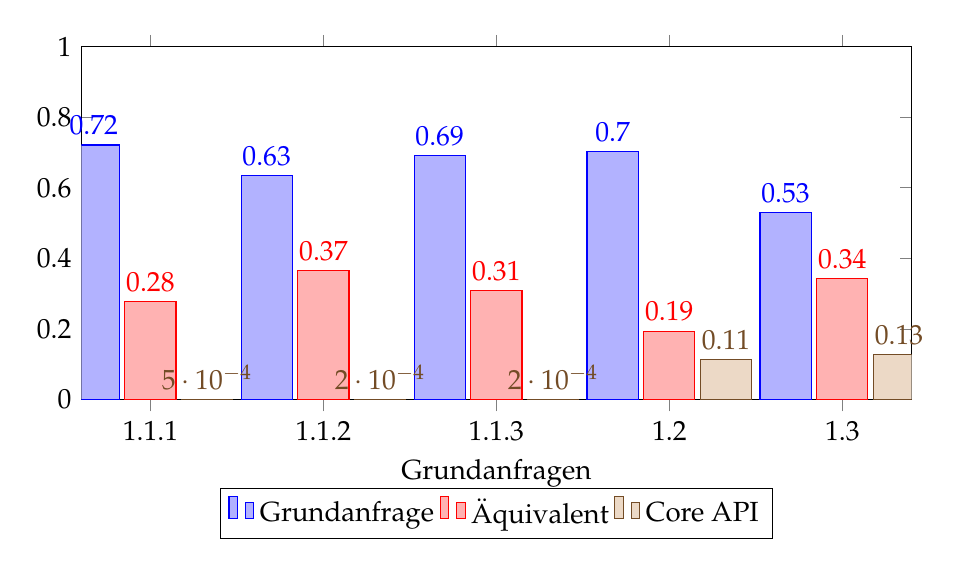
\begin{tikzpicture}
\centering
  \begin{axis}[
ybar,
bar width=.65cm,
width=\textwidth,
height=.5\textwidth,
legend style={at={(0.5,-0.25)},
	anchor=north,legend columns=-1},
symbolic x coords={1.1.1,1.1.2,1.1.3,1.2,1.3},
xtick=data,
nodes near coords,
nodes near coords align={vertical},
ymin=0,ymax=1,
xlabel={Grundanfragen},
]

\addplot coordinates {(1.1.2,0.6345) (1.1.1,0.7211)(1.1.3,0.6908)(1.2,0.7025) (1.3,0.5297)};
\addplot coordinates {(1.1.2,0.3652) (1.1.1,0.2783)(1.1.3,0.3089)(1.2,0.1935) (1.3,0.3434)};
\addplot coordinates{(1.1.2,0.0002)(1.1.1,0.0005)(1.1.3,0.0002)(1.2,0.1139)(1.3,0.1269)};
\legend{Grundanfrage,Äquivalent,Core API}
\end{axis}
\end{tikzpicture}
\captionof{figure}{Übersicht der Anfragen aus dem ersten Testlauf} 
\label{ref:Compare1}
\end{center}
\FloatBarrier

\subsection{Ergebnisse des zweiten Testlaufes}
In der Grundanfrage 2.1.1
\begin{Verbatim}[frame=single]
MATCH(p:Person{name:'Person1'})-[:RELATIONSHIP3*2]->(p1:Person) 
RETURN COUNT(DISTINCT(p1))
\end{Verbatim}
 wurden bei der Traversierung bis zur Tiefe 2 ausgehend von Person1 99 \% aller Knoten des Graphen erreicht. Bei der Tiefe3 wurden alle Knoten erreicht. Wie Tabelle \ref{tab:Query2_1} zeigt, besteht zwischen der Traversierung bis zur Tiefe 2 und Tiefe 3  ein minimaler zeitlicher Unterschied von durchschnittlich ca. 5,6\%, dies widerspricht der Hypothese, dass die Zeit in Cypher doppelt so hoch sein wird. Es besteht so kein direkter Zusammenhang zwischen der Anzahl der zu betrachtenden Knoten und der Bearbeitungszeit. Wie erwartet verändert sich die Berechnungszeit nur minimal bei der Breiten- und Tiefensuche, wenn die Tiefe um 1 erhöht wird.  \newline 
Es wurde bestätigt, dass die Anfrage mit Tiefensuche signifikant schneller als die Anfrage mit Breitensuche ausgeführt wird, in diesem Fall ist die Anfrage für die Tiefe 2 ca. 84\% schneller. Dies wurde in Kapitel 3 durch das Verhältnis der Breite zur Tiefe begründet. 
\FloatBarrier
\begin{table}[h]
\centering
		\begin{tabular}{ |p{3cm}||p{3cm}|p{3cm}|p{3cm}|  }
			\hline
			Anfrage& Cypher & Breitensuche&Tiefensuche\\
			\hline
			Tiefe 2   & 224431    & 1190&  92\\
			Tiefe 3&    234132  & 1278   & 89\\
			\hline
		\end{tabular}
		\caption{Grundanfragen 2.1.1 und 2.1.2}
		\label{tab:Query2_1}
\end{table}
\FloatBarrier
\noindent Wie Tabelle \ref{tab:Query2_2} zeigt, besteht kein  signifikanter Unterschied zwischen Grundanfrage 2.2
\begin{Verbatim}[frame=single]
MATCH t=(p:Person{name :'Person1'})-[:RELATIONSHIP3]->(p1:Person)
-[:RELATIONSHIP3]->(p2)
WHERE NOT (p)-[:RELATIONSHIP3]->(p2) 
RETURN COUNT(DISTINCT(p2))
\end{Verbatim} 
 und der äquivalenten Anfrage in Cypher. Beide Anfragen sind um ein vielfaches langsamer als die Anfrage, die die Core API verwendet. In der Core API Anfrage wurden 2 Ergebnismengen vom Java-typ $Set$ gebildet und durch den Aufruf der Funktion $removeAll()$  wurden die Elementen der einen Mengen aus der anderen Menge entfernt. Dies entspricht einer Realisierung von dem $Where\;not$ Ausdruck  in Java und besitzt eine bessere Performanz. Alle 3 Anfragen besitzen im Vergleich zu vorangegangen Anfragen eine extrem hohen Ausführungszeit.
\FloatBarrier
\begin{table}[h]
	\centering
		\begin{tabular}{ |p{3cm}|p{3cm}|p{3cm}|p{3cm}|  }
			\hline
			Grundanfrage 2.2 & Äquivalent&Core API\\
			\hline
			4740646    & 4753414 &  1609\\
			\hline
		\end{tabular}
		\caption{Grundanfrage 2.2}
		\label{tab:Query2_2}
\end{table}
\FloatBarrier
\noindent Der kürzeste Pfade, welcher in Grundanfrage 2.3
\begin{Verbatim}[frame=single]
MATCH (p:Person{name :'Person1'}),(p1:Person{name :'Person42'}),
path=shortestPath((p)-[:RELATIONSHIP4*..3]->(p1)) 
RETURN LENGTH(path)
\end{Verbatim} 
 untersucht wurde, besitzt die Länge 2. Die Grundanfrage 2.1.1 zeigt, dass bei einer Pfadlänge von 2 die meisten Knoten ausgehend von Person1 erreicht werden. Wie in Tabelle \ref{tab:Query2_3} zu sehen, ist die Ausführungszeit der Anfrage in Cypher unter Verwendung des gegebenen Algorithmus, geringer als alle anderen Grundanfragen außer Grundanfrage 1.2. Erstmalig ist die Anfrage in Cypher schneller als die alternative Formulierung in der Core API. Der relative Unterschied beträgt 37 \% und  der absolute Unterschied 3,1 ms. Durch die geringe absolute Differenz ist es nicht garantiert, dass der kürzeste Pfad mit der Verwendung von Cypher immer die schnellste Schnittstelle darstellt. \newline
Die äquivalente Formulierung in Cypher besitzt die höchste aller beobachtetet Ausführungszeiten mit ca. 2,3 Stunden. Diese Formulierung ist eine naiver Ansatz ohne Verwendung des Algorithmus und besitzt viele Berechnungsschritten, die durch den Algorithmus entfallen würden. Zudem stoppt der Limit-Ausdruck nicht vorzeitig die Berechnung, sondern filtert die Ergebnismenge erst nach der Berechnung, dieses Verhalten ist mit der konservativen Stop-Strategie aus SQL zu vergleichen\parencite{carey1997saying}.   
\FloatBarrier
\begin{table}[!htb]
	\centering
		\begin{tabular}{ |p{3cm}|p{3cm}|p{3cm}|p{3cm}|  }
			\hline
			Grundanfrage 2.3 & Äquivalent&Core API\\
			\hline
			8,4    & 8370298 &  11,5\\
			\hline
		\end{tabular}
		\caption{Grundanfrage 2.3}
		\label{tab:Query2_3}
\end{table}
\FloatBarrier
\noindent Die Ergebnisse der Traversierungen des gesamten Graphen, wie in Grundanfrage 2.4
 \begin{Verbatim}[frame=single]
MATCH (a)-[RELATIONSHIP4]->(b) RETURN COUNT(DISTINCT(b))
\end{Verbatim}
 werden in Tabelle \ref{tab:Query2_4} dargestellt.
 In der Core API ist die einseitige Traversierung mit Breitensuche ca. 4,8\% langsamer als der gleiche Algorithmus bei einer bidirektionalen Traversierung. Bei der Tiefensuche beträgt der Unterschied ca. 13\%. In beiden Fällen sind die einseitigen Traversierungen wie erwartet langsamer als die bidirektionale Alternativen. \newline
Trotz einer semantischen Äquivalenz von Grundanfrage 2.4.1 mit der Grundanfrage 2.1.2, bei der alle Knoten erreicht werden, ist eine signifikant höhere Ausführungszeit zu beobachten. Dieses Verhalten lässt sich nur mit dem Fehlen einer frühzeitigen Abbruchbedingung erklären.    
\FloatBarrier
\begin{table}[!htb]
	\centering
	\begin{tabular}{ |p{5cm}||p{3cm}|p{3cm}|p{3cm}|  }
		\hline
		Anfrage & Zeit\\
		\hline
		Grundanfrage 2.4.1 & 284594\\
		\hline
		Vergleichsanfrage 1 & 31020  \\
		\hline
		Grundanfrage 2.4.2 & 31050\\
		\hline
		Grundanfrage 2.4.3 &  29558  \\
		\hline
		Grundanfrage 2.4.4 &  26982\\
		\hline
	\end{tabular}
	\caption{Grundanfragen 2.4.1-2.4.4}
	\label{tab:Query2_4}
\end{table}
\FloatBarrier

\subsection{Ergebnisse des dritten Testlaufes}
Für die folgenden Aussagen werden die Werte aus der Tabelle \ref{tab:Query3}  betrachtet. Dieses Tabelle stellt die Zeiten der Grundanfragen, ihrer Äquivalente in der Core API und in der OrientDB dar. \newline
Die Grundanfragen 1.1.1-1.1.3 werden in Cypher durchschnittlich ca. 12 mal schneller ausgeführt als in der OrientDB, die relativ langen Bearbeitungszeiten bei beiden Systemen entstehen durch die Bedingungen im Where-Prädikat. In allen Fällen benötigt die Grundanfrage 1.1.3, welche die eingehenden und ausgehenden Kanten betrachtet, die längste Zeit zur Bearbeitung. Im Vergleich zu Neo4j und den anderen Anfragen, die an OrientDB gestellt wurden, benötigen die Grundanfragen 1.1.1-1.1.3 in OrientDB extrem viel Zeit zur Bearbeitung, nur Grundanfrage 2.2 benötigt eine vergleichbar lange Zeit. Dies zeigt, dass OrientDB wie Neo4j durch das Einfügen einer Bedingung im Where-Prädikat sehr stark beeinflusst wird und bei solchen Anfragen eine langsame Berechnung ausführt. \newline
 Grundanfrage 1.2, welche solange über den Graphen traversiert bis ein bestimmter Knoten gefunden ist, weist in OrientDB eine schnellere Bearbeitungszeit als Neo4j mit der Core API oder Cypher auf und wird ca. 3,7 mal schneller bearbeitet als die Anfrage in Cypher gestellt. Die Grundanfragen 2.1.1 und 2.1.2, welche ebenfalls mit einer Abbruchbedingung über den Graphen traversieren, besitzen auf OrientDB ausgeführt auch eine bessere Zeit als Cypher. Daraus lässt sich schließen, dass OrientDB  bei einer Traversierung mit frühzeitigem Abbruch eine bessere Performanz besitzt, als Neo4j unter der Verwendung von Cypher. Bei einer kompletten Traversierung des Graphen wie in den Grundanfrage 2.4.1 und 2.4.2, besitzt Neo4j mit der Core API oder mit Cypher eine bessere Performanz als OrientDB. In Cypher wird die Grundanfrage 2.4.1 ca. 2,7 mal schneller bearbeitet als die gleiche Anfrage in SQL mit OrientDB und mit der Core API wird die Anfrage ca. 27 mal schneller beantwortet. \newline
Grundanfrage 1.3, welche eine einfache Anfrage zum Finden von gemeinsamen Nachbarn darstellt, besitzt in Cypher und der Core API eine relativ geringe Bearbeitungszeit in der Größenordnung von einigen Millisekunden. In OrientDB befindet sich Grundanfrage 1.3 mit einer benötigten Zeit von 83955 ms in einer anderen Größenordnung und deutet darauf hin, dass der Vergleich von 2 Mengen miteinander in Neo4j effizienter implementiert ist. Dies ist auch in Grundanfrage 2.2 zu beobachten, für diese Anfrage muss bis in die Tiefe 2 traversiert werden und 2 Mengen müssen miteinander verglichen werden. Die Anfrage besitzt eine hohe Bearbeitungszeit, obwohl das Traversieren in der Tiefe 2, wie bei Grundanfrage 2.1.1 mit 72092 ms zu beobachten, eine relative geringe Zeit benötigt, der Vergleich der beiden Mengen bildet so den rechenaufwendigeren Schritt. \newline
{\color{red} Ergebnis von 2.1.2 abwarten} Die Traversierungen in den Tiefen 2 und 3, welche durch die Grundanfragen 2.1.1 und 2.1.2 dargestellt werden, besitzen in OrientDB eine geringere Bearbeitungszeit {\color{red} Ergebnis von 2.1.2 abwarten}. \newline  
Mit 37,6 ms benötigt OrientDB bei Grundanfrage 2.3 ähnlich wie Neo4j eine relativ kurze Bearbeitungszeit, dies lässt sich durch eine effiziente Implementierung des shortestpath-Algorithmus erklären. Da das Finden des kürzesten Pfades eine grundlegendes Problem bei Graphen ist, wurde der Algorithmus bereits in der OrientDB Version 1.7.8 vom 13. August 2014 veröffentlicht\footnote{https://orientdb.com/released-orientdb-1-7-8/}. Durch die frühe Zurverfügungstellung ist es wahrscheinlich, dass der Algorithmus mit einer effizienten Implementierung veröffentlicht wurde oder über die Jahre optimiert wurde. \newline
Für die Grundanfrage 2.4.2, welche mit Breitensuche über den gesamte Graphen traversiert, ist nur ein Vergleich zwischen OrientDB und der Core API von Neo4j möglich, da der Such-Algorithmus in Cypher nicht explizit angegeben werden kann und immer Tiefensuche verwendet wird. Durch die gleiche Komplexität von O(V+E) bei der Tiefen- und Breitensuche, benötigen die Grundanfragen 2.4.1 und 2.4.2 in OrientDB ungefähr die gleiche Bearbeitungszeit. In Cypher wird die Grundanfrage 2.4.1 ca. 2,7 mal schneller bearbeitet. Mit Verwendung der Core API wird die einseitige Tiefen- und Breitensuche durchschnittlich ca. 24.8 mal schneller beantwortet als auf OrientDB. Dabei muss berücksichtigt werden, dass die Core API ein hohes technisches Verständnis voraussetzt und nahe an den Kernfunktionen arbeitet und OrientDB die Anfragesprache SQL verwendet, welche eine weniger abstrakte Schnittstelle für den Nutzer darstellt und durch den Abstand zum Kern eine geringere Performanz besitzt. \newline
Insgesamt besitzt die Core API von Neo4j in fast allen Fällen eine signifikant bessere Performanz als OrientDB. Der direkte Vergleich zwischen den Anfragesprachen der beiden Systeme zeigt, dass OrientDB in einigen Fällen, wie dem nicht-vollständigen Traversieren des Graphen, eine bessere Performanz aufweist. Unter der Berücksichtigung aller beobachteten Zeiten besitzen beide Anfragesprachen Stärken und Schwächen, wodurch sich keine allgemeine Aussage über eine bessere Performanz von einer der beiden Sprachen treffen lässt. 
\FloatBarrier
\begin{table}[h]
	\centering
	\begin{tabular}{ |p{6cm}||p{2cm}|p{2cm}|p{2cm}|  }
		\hline
		Anfrage& Cypher & OrientDB & Core API \\
		\hline
	Grundanfrage 1.1.1  & 215383 & 3495459    &  64\\
	Grundanfrage 1.1.2& 212620 & 1674758   & 160   \\
	Grundanfrage 1.1.3& 496704 & 6350806 & 165  \\
	Grundanfrage 1.2& 0,54 & 0,17   & 0,29   \\
	Grundanfrage 1.3 & 8,66& 83955  & 3,2    \\
	Grundanfrage 2.1.1& 224431 & 72092   & 100   \\
	Grundanfrage 2.1.2& 234132& TODO  & 65    \\
	Grundanfrage 2.2& 4740646 & TODO    & 1609  \\
	Grundanfrage 2.3& 8,4  & 37,6   & 11,5   \\
	Grundanfrage 2.4.1& 284594 & 768830  & 31050\\
	Grundanfrage 2.4.2& -  & 774040   & 31020   \\
		\hline
	\end{tabular}
	\caption{Grundanfragen auf Neo4j und OrientDB}
	\label{tab:Query3}
\end{table}
\FloatBarrier
\section{Anwendungsszenario}
Neoj4 Inc. stellt zahlreiche Nutzungen von Graphen in verschiedenen Themenkomplexen vor\footnote{https://neo4j.com/graphgists/ (10.09.18)}. Für jeden Themenkomplex werden mehrere Beispielgraphen von eigenständigen Entwicklern, welche nicht für Neo4j arbeiten, zur Verfügung gestellt. Das folgende Anwendungsszenario stellt den Zweck einer Graphdatenbank für Kinofilme dar.\newline
In diesem Beispiel ist der Nutzer ein Betreiber eines Kinos, welches aktuelle Kinofilm ausstrahlt und besondere Veranstaltungen betreibt. Bei diesen Veranstaltungen werden mehrere Filme von einer Kategorie oder einem bestimmten Schauspieler oder Regisseur gezeigt. Diese Veranstaltungen werden mehrere Wochen vor dem Veranstaltungstermin verplant und finden über mehrere Tage statt. Pro Veranstaltungstag werden im Durchschnitt 4 Filme benötigt. Solche Veranstaltungen wurden schon mehrmals betrieben und die Planung besitzt einen routinierten Ablauf, sodass viele Schritte effizient bearbeitet werden. Der zeitaufwendigste Arbeitsschritt, stellt das Finden von Filmen für das Veranstaltungsprogramm dar. \newline
Aktuell stellt der Kinobetreiber eine Liste mit Filmen für die Veranstaltung manuell zusammen, hierfür werden Filme ausgewählt, die der Betreiber selber kennt und es werden verschiedene Quellen aus dem Internet für eine Auswahl verwendet. Die Liste besitzt die Namen der Filme, zusätzliche Informationen wie Länge sind durch die Vielzahl von Quellen nicht immer vorhanden. Fehlende Informationen müssen für eine optimale Planung des Kinoprogramms erneut herausgesucht werden und einige Filme müssen nach dem initialen Aufstellen der Liste  aussortiert werden. \newline  
Für eine Beschleunigung dieses Arbeitsschrittes kann das Datenbankmanagementsystem Neo4j verwendet werden. Unabhängig von dem Betriebssystem steht die kostenfreie Anwendung $Neo4j\; Desktop$ zur Verfügung. Durch diese Anwendung für den Desktop ist die Bedienung von Neo4j über ein grafischen User Interface(GUI) möglich. Zusätzlich wird die Erweiterung $APOC$ benötigt, welche per Mausklick in $Neo4j\; Dekstop$ eingebunden werden kann. Mit dieser Erweiterung ist es möglich Daten mit verschiedenen Dateiformaten wie CSV in die lokale Neo4j Datenbank zu importieren. Für das Thema Kino stehen im Internet zahlreiche große Datensätze mit Filme kostenfrei zur Verfügung \footnote{https://www.kaggle.com/carolzhangdc/imdb-5000-movie-dataset}. Nach dem Importieren eines solchen Datensatzes, kann der Nutzer durch die Eingabemaske eine Anfrage stellen, um so eine übersichtliche vollständige Liste von Filme zu erhalten. Eine beispielhafte Anfrage in Cypher für eine Liste von Verbrechen-Filmen ist: 
\begin{Verbatim}[frame=single]
MATCH(m:Film) 
WHERE m.Katergorie = Verbrechen
RETURN m.Name as Name, m.Regie as Regie, 
	m.Länge as Länge, m.Plot as Plot 
LIMIT 20
\end{Verbatim}
Diese Anfrage erstellt eine Liste von 20 Filme, die für eine Veranstaltung mit Verbrechen-Filmen passen. Weitere Bedingungen können durch die Cypher Syntax einfach eingefügt werden, beispielsweise wenn gut bewertete Filme von einem Schauspieler gesucht werden:
\begin{Verbatim}[frame=single]
MATCH(s:Schauspieler)-[SpielteIn]->(f:Film) 
WHERE s.Name = 'Peter Dinklage' AND f.Wertung >= 5
RETURN f.Name as Name, f.Regie as Regie, 
	f.Länge as Länge, f.Plot as Plot 
LIMIT 20
\end{Verbatim}
Neo4j übernimmt so das Auswerten von einem Datensatz, der beispielsweise in einem CSV Format dargestellt wird und für den Nutzer schwer zu lesen ist. Durch die effiziente Implementierung von Neo4j wird in kurzer Zeit eine vollständige Liste mit Filmen erstellt, die geforderte Bedingungen erfüllen. Der Arbeitsschritt zum Erstellen einer Liste mit geeigneten Filmen wird damit stark beschleunigt und effizienter ausgeführt.
\section{Limitierungen und zukünftige Arbeit}
Die durchgeführte Evaluation nutzt mit OrientDB  eine einzige Referenzdatenbank. Dies ist keine reine GDB und unterstützt weitere Typen von Datenbanken. Für eine näherer Einordnung der Performanz von Neoj4 ist ein Vergleich mit einer reinen GDB wie beispielsweise der Sparksee Database sinnvoll\footnote{http://www.sparsity-technologies.com/ (28.08.19)}. Diese Datenbank konnte in dieser Evaluation auf Grund von Kommunikationsprobleme mit Sparsity technologies nicht verwendet werden. Durch einen Vergleich mit der Sparksee Database könnte die Performanz von zahlreichen Graphalgorithmen   wie zum Beispiel Zentralitäts-Algorithmen überprüft werden. Dies ist mit OrientDB nicht direkt möglich, da keine vergleichbare Implementierung der von Neo4j unterstützen Graphalgorithmen im vollen Ausmaß in OrientDB gegeben ist. \newline 
Ein Vergleich zwischen Neo4j und einer relationalen Datenbank, wie in \parencite{vicknair2010comparison} beschrieben, ist für eine weitere Beschreibung der Vor- und Nachteile einer Graphdatenbank sinnvoll. Dieser Vergleich wurde aus zeitlichen Gründen nicht vollzogen. Die Referenz zur OrientDB hat einen Vergleich zu einer anderen noSQL-Datenbank dargestellt und so ein erste Einschätzung zu der Performanz von Neo4j ermöglicht. \newline
Ein weitere Aspekt der betrachtet werden kann, ist das Ausführen von Neo4j im Server Modus und auf mehreren Geräten verteilt. Durch diesen Aspekt können die ACID und CAP Eigenschaften genau untersucht werden und die Grenzen einer verteilten Neo4j-Datenbank getestet werden. Zudem kann ein Vergleich zwischen der Datenbank im eingebetteten Modus und dem Server Modus durchgeführt werden. So können genaue Vor- und Nachteile und ein Anwendungsszenario spezifiziert werden. \newline
Eine kleinerer nicht betrachteter Aspekt ist die temporale Eigenschaft von Neo4j. Der vorgestellte Datensatz besitzt Attribut vom Typen $Date$ und stellt so eine temporale Datenbank dar, doch es fehlt ein Testlauf mit Anfragen zu diesem Attribute. Eine Allgemeine Betrachtung des temporalen Verhalten der Datenbank ist für eine genauere Einordnung von Neo4j im Vergleich zu anderen temporalen Graphdatenbanken sinnvoll. 
\section{Fazit}
Neo4j unterstützt mit den Java-Standardtypen und zahlreichen zeitlichen Typen wie $Time$, $LocalTime$ oder $DateTime$ eine Vielzahl von Datentypen, welche für die Modellierungen von Daten notwendig sind\footnote{https://neo4j.com/docs/cypher-manual/current/syntax/values/ (28.08.19)}. Durch die Zurverfügungstellung der Anwendungen $Neo4j\; Dekstop$ und $Neo4j\; Browser$ und einer dazu gegebenen Anfragesprache, werden die benötigten Kenntnisse zur Bedienung des System minimiert. Für eine spezifischeren Gebrauch der Datenbank, werden mehrere Programmiersprachen unterstützt. Durch diese Schnittstellen ist es mögliche, das System auf viele Weisen zu nutzen und eine große Zielgruppe kann das System für viele Szenarien verwenden. \newline 
Testlauf 1 und 2 zeigen, dass der Gebrauch der Java Core API in allen Fällen zu einer signifikant besseren Performanz führt. Mit Verwendung der Traversal API besitzt der Nutzer eine flexible Möglichkeit die Performanz seiner Anfragen zu beeinflussen. Zum Beispiel ist es möglich zwischen Breiten- und Tiefensuche zu wählen. Die am schnellsten bearbeiteten Anfragen besitzen keine gemeinsame Kategorie von den vorgestellten Kategorien aus Absatz \ref{Kategorien}. Die am langsamsten bearbeiteten Anfragen besitzen ebenfalls keine gemeinsamen Kategorien. Grundanfrage 2.2.1, welche die einzige Mustervergleichs-Anfrage ist, besitzt eine besonders hohe Ausführungszeit. Dementsprechend lässt sich nur für Mustervergleichs-Anfragen ein Bezug von Anfragen-Kategorie und Performanz in Neo4j erkennen, die anderen Kategorien weisen keinen solchen Bezug auf. \newline
Wie die Tabellen \ref{tab:Query1_2} und \ref{tab:Query2_3} zeigen, können semantisch gleiche Anfragen in Cypher Unterschiede in ihrer Performanz aufzeigen. Dieses Verhalten ist in den APIs ebenfalls zu beobachten. Das System lässt sich durch eine hohe Anzahl von Schnittstellen leicht benutzten, aber das System effektiv zu nutzen und eine Anfrage effizient ausführen zu lassen, ist nicht trivial und erfordert technologische Kenntnisse. Durch Hinweise von Neo4j Inc. werden einige Möglichkeiten für das effiziente Ausführen gegeben \footnote{https://neo4j.com/blog/tuning-cypher-queries/ (07.08.19)}. Diese Hinweise befassen sich teilweise mit dem Umformulieren der Anfragen, um das volle Potenzial des Optimierers nutzen zu können. Wie in den Ergebnissen zur Grundanfrage 1.2 erläutert, deutet dies unter anderem auf einen unperformanten Optimierer hin. \newline
Im Vergleich zu der Muli-Model Datenbank OrientDB unter Verwendung von SQL besitzt Neo4j mit der Core API ein signifikant bessere Performanz. Mit  Anfragesprache Cypher ist die Performanz von Neo4j nicht mehr eindeutig besser. Der verwendete Datensatz ist unter Neo4j ca. 58 \% größer, als bei OrientDB. Allgemein besitzt Neo4j so eine bessere Performanz, wenn die Kenntnisse durch den Nutzer gegeben sind, aber die Speicherverwaltung unter Neo4j ist schlechter. Wie die Performanz im globalen Kontext im Vergleich zu mehreren anderen Datenbankmanagementsystemen ist, wie in \parencite{jouili2013empirical} ausgeführt,  lässt im Rahmen dieses Experiments nicht sagen. 


%\include{Chapters/Chapter4} 
%\include{Chapters/Chapter5} 

%----------------------------------------------------------------------------------------
%	THESIS CONTENT - APPENDICES
%----------------------------------------------------------------------------------------

\appendix % Cue to tell LaTeX that the following "chapters" are Appendices

% Include the appendices of the thesis as separate files from the Appendices folder
% Uncomment the lines as you write the Appendices

%\include{Appendices/AppendixA}
%\include{Appendices/AppendixB}
%\include{Appendices/AppendixC}

%----------------------------------------------------------------------------------------
%	BIBLIOGRAPHY
%----------------------------------------------------------------------------------------

\printbibliography[heading=bibintoc]

%----------------------------------------------------------------------------------------

\end{document}  
